\documentclass[12pt]{article}
\usepackage[english]{babel}
\usepackage{natbib}
\usepackage{pdfpages}
\usepackage{float}
\usepackage{url}
\usepackage[utf8x]{inputenc}
\usepackage{amsmath}
\usepackage{graphicx}
\graphicspath{{images/}}
\usepackage{parskip}
\usepackage{fancyhdr}
% \usepackage{vmargin}
% \setmarginsrb{2 cm}{2.5 cm}{2 cm}{2.5 cm}{1 cm}{1.5 cm}{1 cm}{1.5 cm}
\usepackage[a4paper,left=2.5cm,right=3cm]{geometry}
\addtolength{\topmargin}{-0.5cm}
% \setmarginsrb{3 cm}{2.5 cm}{3 cm}{2.5 cm}{1 cm}{1.5 cm}{1 cm}{1.5 cm}

\title{Workshop on Spoken Dialogue Systems for PhDs, PostDocs and New Researchers}								% Title
% \author{Chong Hui Yong}								% Author
\date{September 16, 2016}											% Date

\def\EDITION{{12}}  % 12 was for 2016 workshop

\newcommand\textbox[1]{%
      \parbox{.333\textwidth}{#1}%
}

\makeatletter
\let\thetitle\@title
% \let\theauthor\@author
\let\thedate\@date
\makeatother

\pagestyle{fancy}
\fancyhf{}
\lhead{\thetitle}
\cfoot{\thepage}

\begin{document}

%%%%%%%%%%%%%%%%%%%%%%%%%%%%%%%%%%%%%%%%%%%%%%%%%%%%%%%%%%%%%%%%%%%%%%%%%%%%%%%%%%%%%%%%%

\begin{titlepage}
	\centering
    \vspace*{0.1 cm}
    
\includegraphics[scale = 0.8]{yrrsds_logo.png}\\[1.0 cm]
    \textsc{\LARGE ICT, Los Angeles, USA}\\[2.0 cm]
	\textsc{\Large Proceedings 2016}\\[0.5 cm]
	\rule{\linewidth}{0.2 mm} \\[0.4 cm]
	{ \huge \bfseries \thetitle}\\
	\rule{\linewidth}{0.2 mm} \\[1.0 cm]

\begin{figure}[H]
\centering
    % TODO sponsors
    
\includegraphics[scale=0.4]{yrrsds_logo.png} \\
\end{figure}

	{\large \thedate}\\[2 cm]
\end{titlepage}


\section*{Foreword}
The Young Researchers Roundtable on Spoken Dialog Systems (YRRSDS) has been for many of us our first encounter with life in the research world. It aspires to be an environment in which young researchers can present late-breaking work, discuss ideas, connect with other researchers, and hear first person accounts of what it means to be a part of this field straight from respected senior members in the industry and academy.

There is an additional angle that is often overlooked, which is that YRRSDS is also the perfect stepping stone for anyone newly entering this field. Before the “big league” conferences, YRRSDS serves as an ideal forum for young researchers to discuss ideas in a laid-back setting with others who may have as many doubts and questions. This circulation of fresh perspectives has the potential for great impact on the next generation of research. The Roundtable’s focus has always been to foster creative thinking and strengthen an international network of researchers. Past, present, and future YRRSDS participants form a pipeline of mentors and colleagues as former YRRSDS become senior professionals themselves. We are proud to be part of the chain of young researchers carrying these ideals into the present day.

We hope you enjoy the Roundtable. It’s been a privilege for us to host its \EDITION th edition, and it’s our honor to have you join us. If you take away from YRRSDS as much as we have, we encourage you to volunteer for organizing next year’s YRRSDS to keep the torch moving towards the future.

\hfill {\bf The YRRSDS \the\year \ committee}
\pagebreak

\section*{Organizing Committee}

\begin{itemize}
\item Alexandros Papangelis, Toshiba CRL
\item David Cohen, Carnegie Mellon University
\item Eli Pincus, University of Southern California
\item José David Lopes, KTH Royal Institute of Technology
\item Ondřej Plátek, Charles University in Prague
\item Lu Chen, Shanghai Jiao Tong University
\item Maria Schmidt, KIT Karlsruhe Institute of Technology
\item Ramesh Manuvinakurike, University of Southern California
\item Tiancheng Zhao, Carnegie Mellon University
\item Zhou Yu, Carnegie Mellon University
\end{itemize}

\section*{Advisory Committee}

\begin{itemize}
\item Srinivas Bangalore, Interactions (former AT\&T Research)
\item Luciana Benotti, Universidad Nacional de Córdoba
\item Rolf Carlson, KTH Royal Institute of Technology
\item Maxine Eskenazi, Carnegie Mellon University
\item Kallirroi Georgila, University of Southern California
\item Jim Glass, Massachusetts Institute of Technology
\item Kristiina Jokinen, University of Helsinki
\item Tatsuya Kawahara, Kyoto University
\item Diane Litman, University of Pittsburgh
\item Wolfgang Minker, University of Ulm
\item Sebastian Möller, Technische Universität Berlin
\item Mikio Nakano, Honda Research Institute
\item David Schlangen, Universität Bielefeld
\item Gabriel Skantze, KTH Royal Institute of Technology
\item David Traum, University of Southern California
\item Nigel Ward, University of Texas at El Paso
\item Jason Williams, Microsoft Research
\item Steve Young, University of Cambridge
\item Oliver Lemon, Heriot-Watt University
\item Alex Lascarides, University of Edinburgh
\item Sungjin Lee, Yahoo!
\item Timothy Bickmore, Northeastern University
\item L P Morency, Carnegie Mellon University
\item David DeVault, USC Institute for Creative technologies
\item Matthew Purver, Queen Mary University, London
\item Julia Hirschberg, Columbia University
\item Deepak Ramachandran, Nuance Communications
\item Svetlana Stoyanchev, Interactions Corporations
\end{itemize}
\pagebreak

%%%%%%%%%%%%%%%%%%%%%%%%%%%%%%%%%%%%%%%%%%%%%%%%%%%%%%%%%%%%%%%%%%%%%%%%%%%%%%%%%%%%%%%%%

\tableofcontents
\pagebreak

%%%%%%%%%%%%%%%%%%%%%%%%%%%%%%%%%%%%%%%%%%%%%%%%%%%%%%%%%%%%%%%%%%%%%%%%%%%%%%%%%%%%%%%%%

\section{Invited talks}
\subsection{Natural Language Generation for Dialogue Systems: What we (still) don't know. Marilyn Walker, UC Santa Cruz}
Abstract:  Dialogue interaction provides an extremely challenging and grounded evaluation of natural language understanding. Natural language understanding has greatly improved over the last 20 years, but what level of understanding is needed to respond appropriately in dialogue in a particular context? How can natural language generation produce these contextually appropriate responses? How can it scale? Should a conversational assistant have a persona or style? Should it entrain to the user, take the initiative, understand greetings and other phatic acts, and use an explicit model of dialogue structure? What are some near term and some
long term solutions towards more natural dialogue interaction?

\subsection{Stefan Scherer (USC ICT)}
\subsection{Gokhan Tur (Google Research)}

\section{Roundtables}
The discussions are the core reason to held the workshop.
They tend to be informal, futuristic and sometimes funny.
The notes taken by the organizers is a subjective attempt to capture some conclusions.


% \subsection{Evaluating Chatbots}
% \begin{itemize}
% \item crowd-source appropriateness of next response
% \item Stefan Ultes explored interaction quality
% \item Ryan - next utterance classification - is not perfect but better than Bleu
% \item David Traum
%     \item coherence is not bad - quite correlate with user satisfaction
%     \item permuted turn in dialogues
%     \item multiple Wizards of Oz
% \item turn by turn measures
%     \item may be combined to global measure which is needed for chatbot
% \item ask Tony
%     \item DialPort evaluation platform (not only for chatbots) http://arxiv.org/abs/1606.02562
% \item Marilyn suggest preparing shared-tasks for chatbot
%     \item 10 years of Big Bang theory transcription as training data
% \item appropriateness vs coherence
%     \item appropriateness
%         \item not much like dialogue
%         \item is very situation dependent
% \item play it safe - is it desired?
%     \item future expectation?
%     \item do not repeat too often
% \item summarize context
%     \item desired especially if the user do not listen much
%     \item propose next context
% \item we should focus on what user wants - task oriented vs chit-chat
%     \item dialogue length is good measure
% \end{itemize}



% \subsection{Advances in Statistical Methods for SDSs}
% - Introduce noise to data and non-cooperative users
%     - branch of after introducing introducing noise
%     - multi-language embeddings
%     - dialogue deep


\subsection{Panel Discussion}

{\it Ethan:} Most meaningful thing was internship. Working in industry and seeing that dreams of doing things which were industry experience. Everything doesn’t materialize.

{\it Traum:} Everything doesn’t materialize. Can you succeed as a student, researcher, find funding source etc. Any answers to those are meaningful.

{\it Walker:} Do something and knowing a lot more in next three months, I will know more. If it doesn’t work, then it can be a baseline. So, working on things and making it better is the goal.

{\it Trung:} Learning many skills is important. Finding dialogue solutions on existing problems is hard. First success was applying a well know method to some other problem. That helps build credibility.

{\it Gokhan:} Cannot become a good researcher sitting at home. People were afraid to try new things. “Standing on shoulders of giants” is meaningful. Environment is meaningful.

\subsubsection*{How to deal with frustrations?}

{\it Walker:} Dialogue picked me and I didn’t pick dialogue. There was a point in time around 2000s when I thought that web access and smartphone was the best. I was worried that my research will all go waste. I didn’t do something else. So, I had to be patient.

{\it Ethan:} Neural nets have been here for quite some time. But, got attention later.

{\it Walker:} Having patience is important. Its like an obsession. Its like doing art. Found analyzing human-human dialogue when SDS didn’t work. So, I kept the motivation going. Started working with social media.

{\it Gokhan:} Don’t follow the trend. Focus on the approach. Know that people are more interested in approach and the results. Results can be obtained with the approach. Build good approach.

{\it Traum:} Spoken vs text based dialogue. Text based was worked on in 80s. But, if ASR came in it would become irrelevant. Now we have a lot of things. Texting isn’t going anywhere. It is not necessarily that it is important to pick and choose what I am really interested in. Pick the best tools for the task and don’t pick the trend

\subsubsection*{How to implement dialogues into the real world?}

{\it Ethan:} Its hard for people to understand the under the hood things. How to incorporate business rules into the things is important. Understand the customer. SDS are target understanding. The challenge is the wall garden. Users are exploring in the dark.

\subsubsection*{Can the users be told what to do?}

{\it Gokhan:} Let users explore. Do more and more thing.

{\it Truam:} Go back to human conversation and see how to converse. You don’t go to McD and ask about integral calculus. So, there is an environment and the reason the system is built for. Give people a chance to explore the system and let them know what the system is built for. Draw on those models. How do you detect that the dialogue is not going anywhere and how to gracefully recover from there?

{\it Walker:} Human in the loop can work?

{\it Ethan:} Not ideal. It’s a hard strategy to work around this problem. Humans could do better.

\subsubsection*{How would you hire someone to work with you?}

{\it Traum:} Depends on the expertise from the people.

{\it Gokhan:} Deep learning

{\it Traum:} (Convert dialogue into a machine learning problem. Not good)

{\it Walker:} Broad coverage people are important. Inquisitive mind and someone who you can talk to about anything. Problem is that broad coverage has to be learnt from the right place. Finding those hard places is hard. Read a lot! Interest in sensitivity to language. Language is a way of communicating and not just a signal.

{\it Ethan:} needs a good judgement. I don’t know is not an answer. Creating new things with all the recent tools is important. Look to learn as much as possible.

\subsubsection*{What is the ideal time and number of people?}

{\it Walker:} 5-6.

{\it Trung:} 30 lot of different expertise.

{\it Traum:} Depends on the kind of dialogue system.

{\it Traum:} we’re focused on language and a few people know a lot about language and more than us, but their contribution as a body of material to us is not quite useful. People from different discipline don’t look at the problem the same way.

{\it Walker:} Lot of times people things everyone can do their own job. Miss out on lot of fun if you don’t have technical skills if you can’t do recent machine learn things. Ex: people can’t contribute to the team if they’re working on a different team. Its important that people are broad in their interest because they may fail to assimilate into different team culture.

\subsubsection*{What should deep learning people do to be accepted into dialogue community?}

{\it Ethan:} give an example. Motivate well.

{\it Marilyn:} think hard about the baselines. Ask people about a good baseline. Ask people what side the issues are on. Have a good baseline for your tasks. Important to keep thinking about the problem and how you set it up.

{\it Gokhan:} happens in ML, my number is so much better is less influential. What was your contribution to make the model better ? How did your contributions affect the numbers ?

{\it Trung:} Deep learning cannot explain why it is better, and this is the reason why it works better and this is a good solution.

\subsection{Roundtable: Commercial SDS}

Two major categories in SDS:
\begin{itemize}
    \item Eliminates labor: remove labor and provide utility. Replacing worker
    \item Ecosystem type: Siri etc. Makes apple’s products more lucrative.
    \item Maluba: Agree with the notion.
    \item IOT provides lot number of use cases. Ex: ATT system, connected dialogue systems.
    \item Ondrej: May be it is not dialogue, may be integration system. Navigation system should ask questions.
\end{itemize}

Commercial dialogue systems are task oriented usually. AI in a game, playstation, talking to the AI and all work in a team. Entertainment system.

\begin{itemize}
    \item Is siri a dialogue system ?
    \item Lacks states. May be it is a question answering system. Not a dialogue.
    \item But, it breaks the question down into multiple questions, so it is a dialogue system. QA system: rudimentary dialogue system. Proof by induction. So, it is a basic SDS. They have voice search. Maintain states and context.
\end{itemize}

Omilia: lot of customers. Conversational systems do not eliminate jobs. Goal is to not lose jobs but change jobs. Time is what matters. Orient agents to provide better customer experience.

Human in the loop AI can help leverage more complex stuff from humans.

Activation of card 2.5 euros cost if humans do the job. Agents can have a call and costs around 0.2 or 0.3. There is a major cost reduction.

Agents need to be able to grab attention. Lot of people just speak and are distracted. So, it doesn’t quite grab attention.

Context of the dialogue: Ex: Hello .. customer missed it .. Hello again. Make the customers move on.
If agent is confined to just finish conversation in a time bound manner, it cannot achieve the goal of optimality.

Customer service: dealing with a person is indivudial. But, the company cares about volumes serviced. How busy the queue.

Having a persona can help businesses perform better.

Imagine building a SDS for fridge, Task oriented system can be deployed without persona. It is like a siri use case.

People like talking to people. Siri: depends on use case.

Security systems should be smart: Robotic dog for security.

IOT: Fridge, camera and all the devices. Eco-systems creation with SDS.

People attribute personality to a voice. Even Roomba is associated a personality. Automatic systems is associated personality.

Alexa with hands free functionality is good and things don’t quite need a personality yet.

Personality is probably needed not in the case where the functionality performs well but when it doesn’t do well ? “I am sorry I didn’t catch that” repeatedly saying is not a good solution and needs a personality.

How to recover from errors is important in commercial vs research sds ? Siri: default is google search.

In Europe customers have completely different attitude to the system.

As soon as they hear system they start swearing.
Demographics might be important.
Status of the customer is quite important to understand the logic.
Learn from data coming in: Data and the systems need to be trained dynamically. The systems can learn from the data that they have already been input. How do these interactions adapt to the new kinds of data coming in?


\subsection{Roundtable: Multi-modal Generation}
Various channels that convey information
How can we combine appropriate channels of information to convey multi-layered information (e.g. say something and indicate uncertainty via non-verbal signals)
Feedback on generated output?
Synchronization of output signals
When do we actually need multiple modalities?
How could MMG affect the way people communicate with the system?

Charts, graphs, other modalities besides just virtual agents; that is also MM generation
Complementarity vs redundancy
We can make some channels more concise if we use more (e.g. verbal \& visual)
Temporal sequences are different for different modalities but need to be coordinated somehow
FML \& BML for non verbal understanding and generation, NVBG, BEAT, CEREBELA
Robots have other constraints, but VA may also be unnatural because they do not adhere to real laws of physics
Output from various modalities may (collectively) be disruptive rather than helpful and we need to design methods of handling All these modalities (e.g. machines in a hospital - all are useful but together they are very noisy)
Some modalities are more urgent / invasive than others (e.g. phone buzzing)
What things matter in evaluating MMG? appropriateness, naturalness - different for different communities - perhaps measure how much people mimic the system
For synchronization, we may have something that enforces rules, e.g. lipsync
Most existing systems start with one channel and then augment it with other channels, rather than generating everything in parallel.

\subsection{Roundtable: Multi-modal Understanding}

\begin{itemize}
    \item Various levels of understanding
\item SLU, Non-verbal behaviour understanding
\item How should we define the various levels of understanding?
\item Can the various modalities be processed separately or not?
\item Understanding based on long-term and short-term knowledge
\item Synchronisation of signals
\item Privacy issues - what kind of information do we keep / ignore?
\end{itemize}

{\bf Notes:}

The fact we don’t understand the French intonational patterns doesn’t allow us to understand

Data is available, is little addressed in current dialogue systems

Needed for annotated data, lack of agreement between annotators

What multi-modal interaction: eye gaze in multi-party gazes.

Intonation as to complete the information of the asr.

Multi-modal understanding is dependent on the end goal.

Synchronize data: ping messages to synchronize time between machines. Latency is not often the same and currently is difficult to address in real time.

Feature representation is still a challenge.

Problem about synchronizing, there is a lot of data available but it is hard for processing the data. Lack of uniformity of in the way the data is collected. Take all the information that we want from one channel is hard. Timeline software that allows analysing all the streams: ELAN.

\subsection{Roundtable: Evaluating Chatbots}

crowd-source appropriateness of next response
Stefan Ultes explored interaction quality
Ryan - next utterance classification - is not perfect but better than Bleu
David Traum
coherence is not bad - quite correlate with user satisfaction
 permuted turn in dialogues
 multiple WoOz
Turn by turn measures
 may be combined to global measure which is needed for chatbot
Ask Tiancheng (Tony)
DialPort evaluation platform (not only for chatbots) http://arxiv.org/abs/1606.02562
Marilyn suggest preparing shared-tasks for chatbot
10 years of Big Bang theory transcription as training data
appropriateness vs. coherence
appropriateness
not much like dialogue
Is very situation dependent
Play it safe - is it desired?
future expectation?
do not repeat too often
Summarize context
desired especially if the user do not listen much
propose next context
We should focus on what user wants - task oriented vs chit-chat
dialogue length is good measure

\subsection{Roundtable: Statistical Method for SLU}

- Has bunch of data labeled. Whats the best way to add new labels ? Slots and intent mapping. How addition of intents and slots? Needs recollecting and re-implementing the pipeline. May be generative models can be a solution to this. Needs re-training.

- Including context into the language understanding.

- Small labeled dataset, but large unlabeled dataset. Using self-taught learning.

- Using annotations on the ASR engine.

- DSTC2 data is static. Variability in the new data. Much more different from the dynamic data. So, SLU needs a service? Problem conversion between state tracking vs understanding.

- SLU: task oriented setting and slot fitting. Interested in non-task oriented setting? Understand what the person is speaking in open domain and respond differently. SLU task is much vague and depends on the domains.

- Generic understanding: AMR: Abstract meaning representation is more powerful than framenet.

- Spoken vs written: written is much harder because its harder to parse. But, spoken have shorter length and easier to parse.

- Give me a perfect AMR parser, but how to build the perfect SDS.

- Opentable API has three variable API. Query to the API which can fulfil the user request.

- Classification is over-simplified version of SLU.

- High precision grammar: disfluencies: Disfluency clean up doesn’t clean up. Query rewrite is a big issue.

- Query rewrite is very dominant. Synonyms and disjunctions are added.

- Query rewrite: Speech is taken as a commodity.

- Incremental SLU could handle works by having barge-ins. Annoying but works. Query success tasks increased by performing incremental SLU.

- Retrain on real user utterances. Corpora is important.

- Residual nets are may be equivalent to RNN. Skipping layers and resnets don’t quite have the same appeal due to depth and randomness.

- Wavenet: generates signals. Wavenets vs resnets ? Generating words is very different from generating images. Could still work. Recursive neural networks.

- Fit to the API is important. -Show me movies of “James Cameroon”- Build trees based on parse tree. Recursive neural networks needs a more structured training data.

- Recursive NN was more linguistically motivated.

- Bracketed representation and LSTM provides the structure.

- Memory augmented neural networks: Memory augments the learning by integrating context.

- Attention models vs memory networks.

- Memory networks are may be better suited for QA and not really dialogue.

- Direct linking works well for parsing lattices.

- Input layer is in the form a lattice. [wordlets]

- Memory networks [QA system] FB data set. Could be a good pointer. Memory network to represent the context.


\section{Position papers}

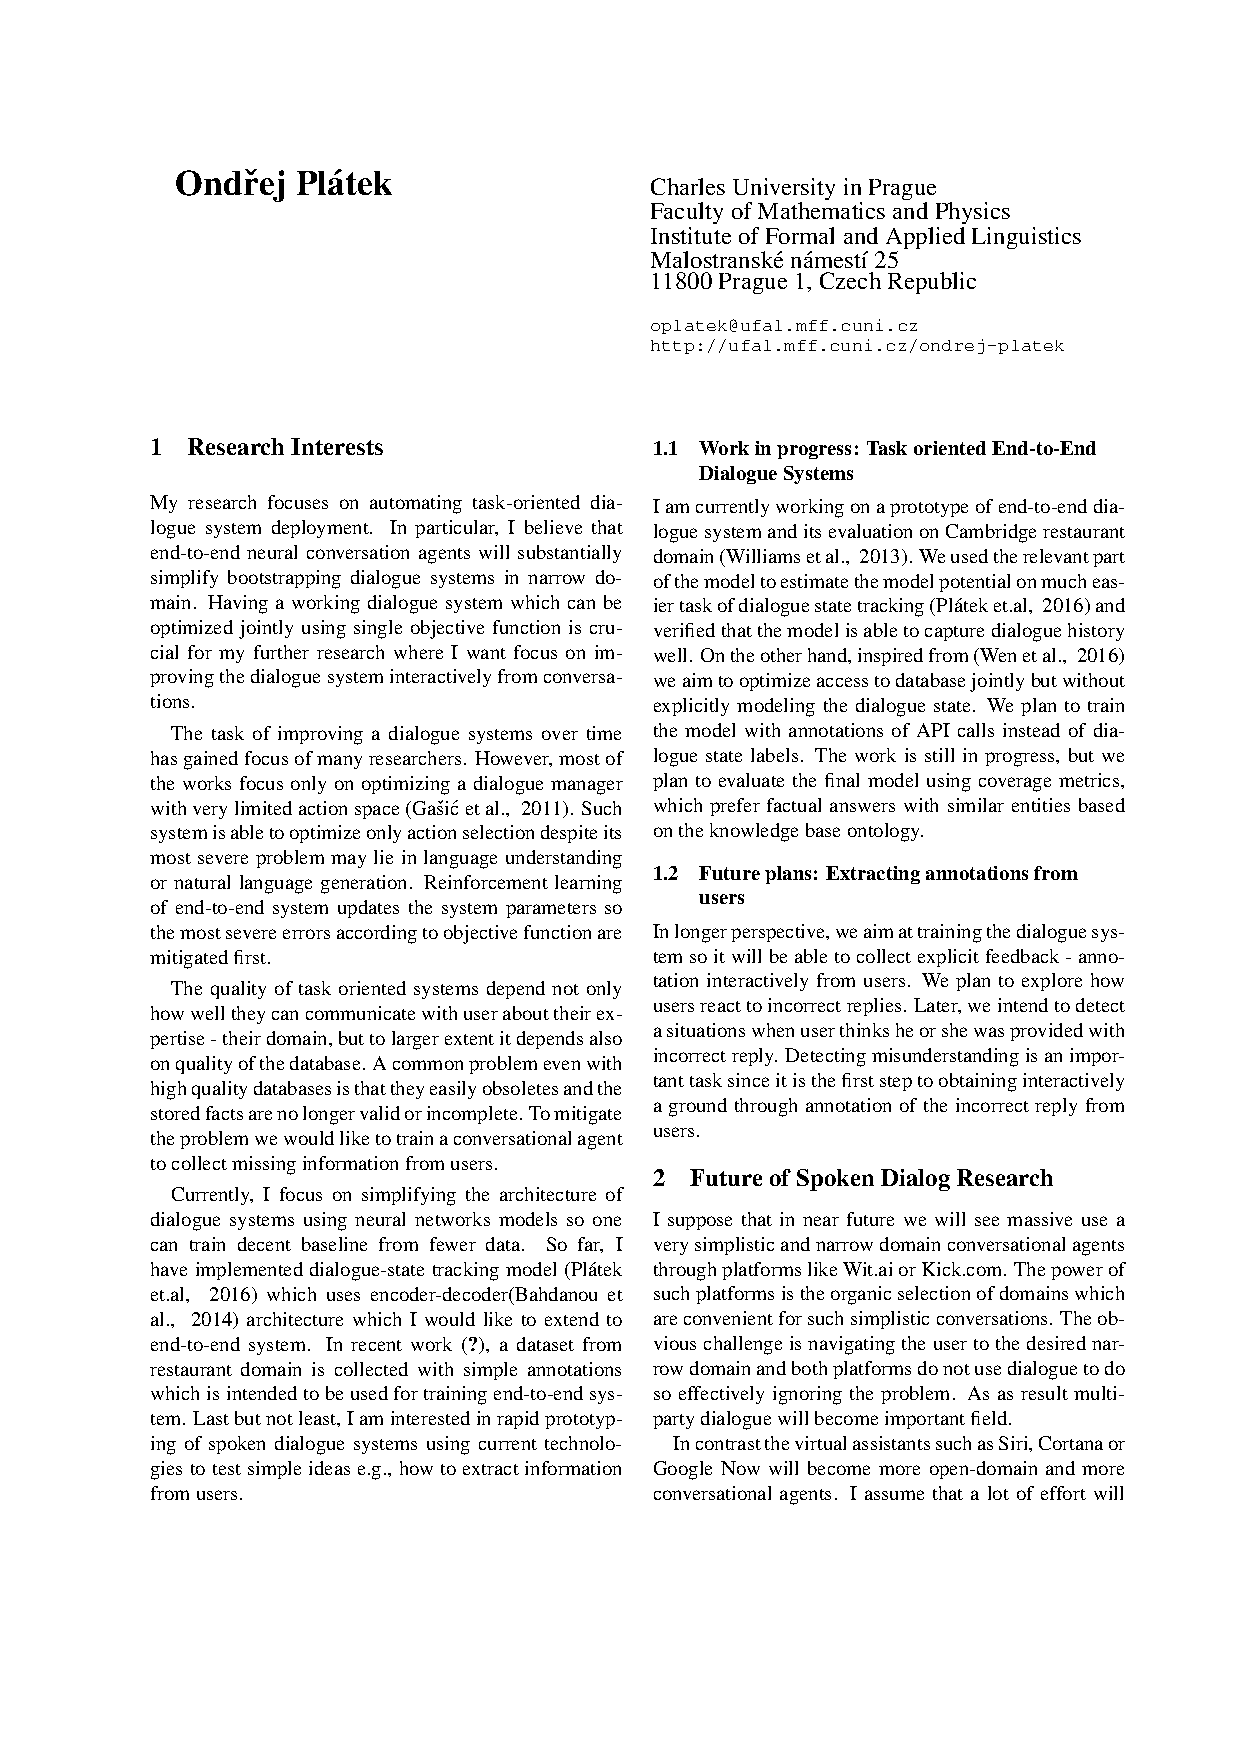
\includepdf[pages=-,pagecommand={}]{YRRSDS_2016_paper_1_ondrej_platek.pdf}
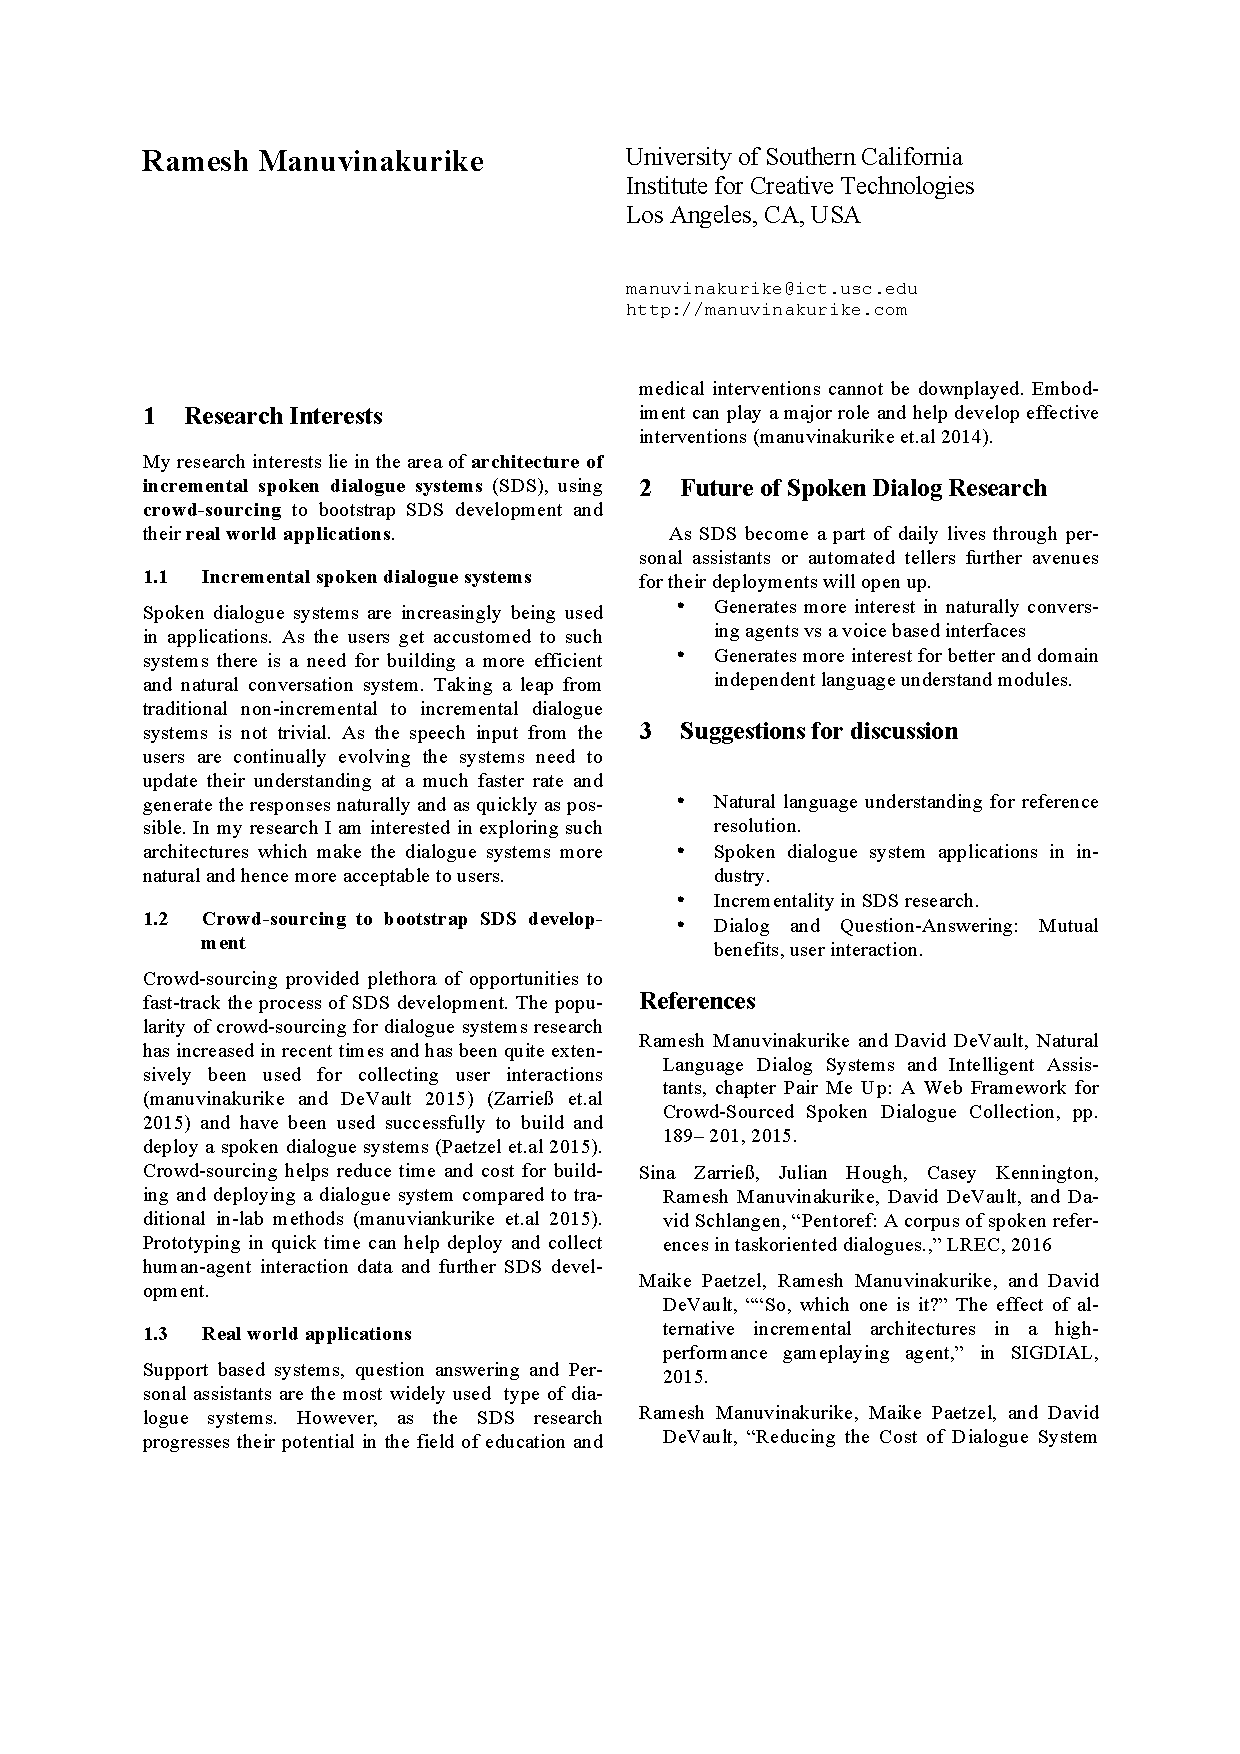
\includepdf[pages=-,pagecommand={}]{YRRSDS_2016_paper_2_remesh_manuvinakurike.pdf}
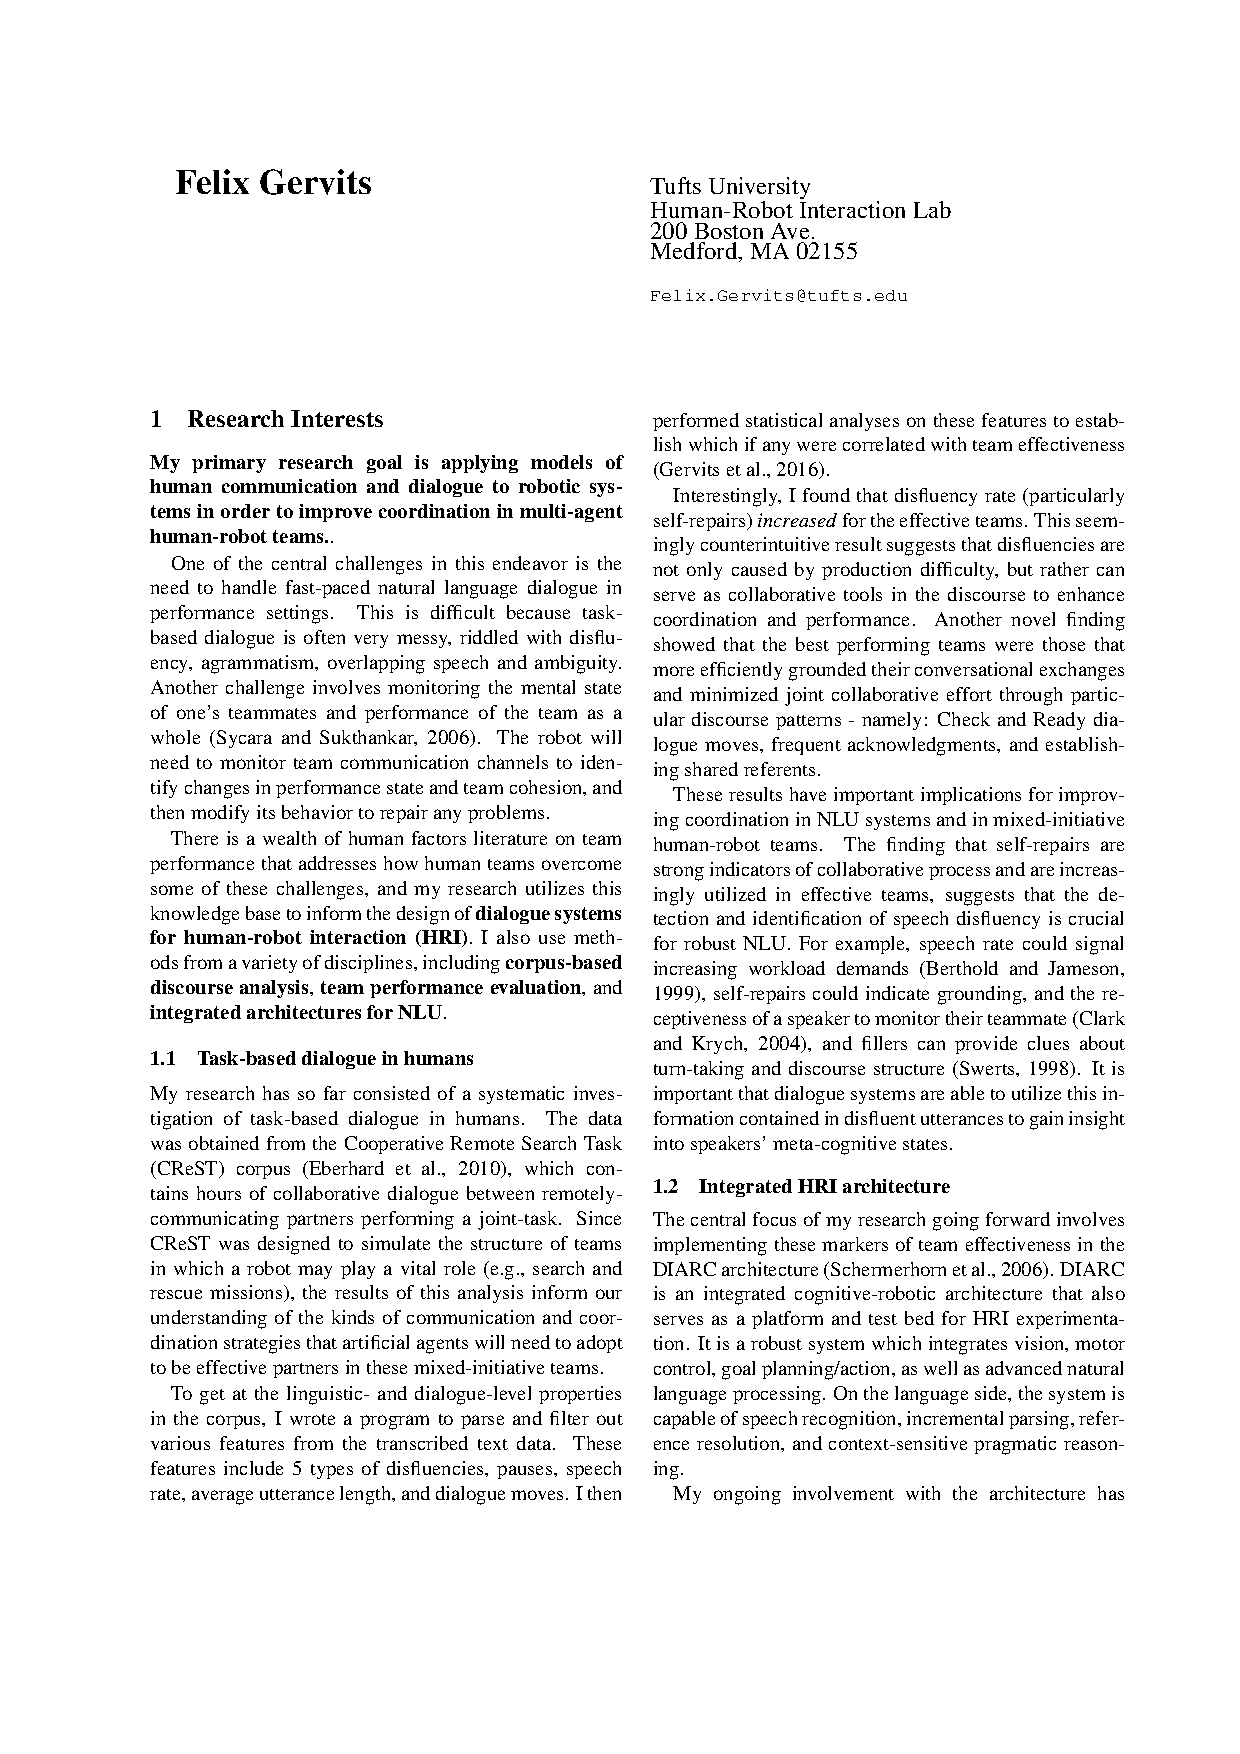
\includepdf[pages=-,pagecommand={}]{YRRSDS_2016_paper_3_felix_gervits.pdf}
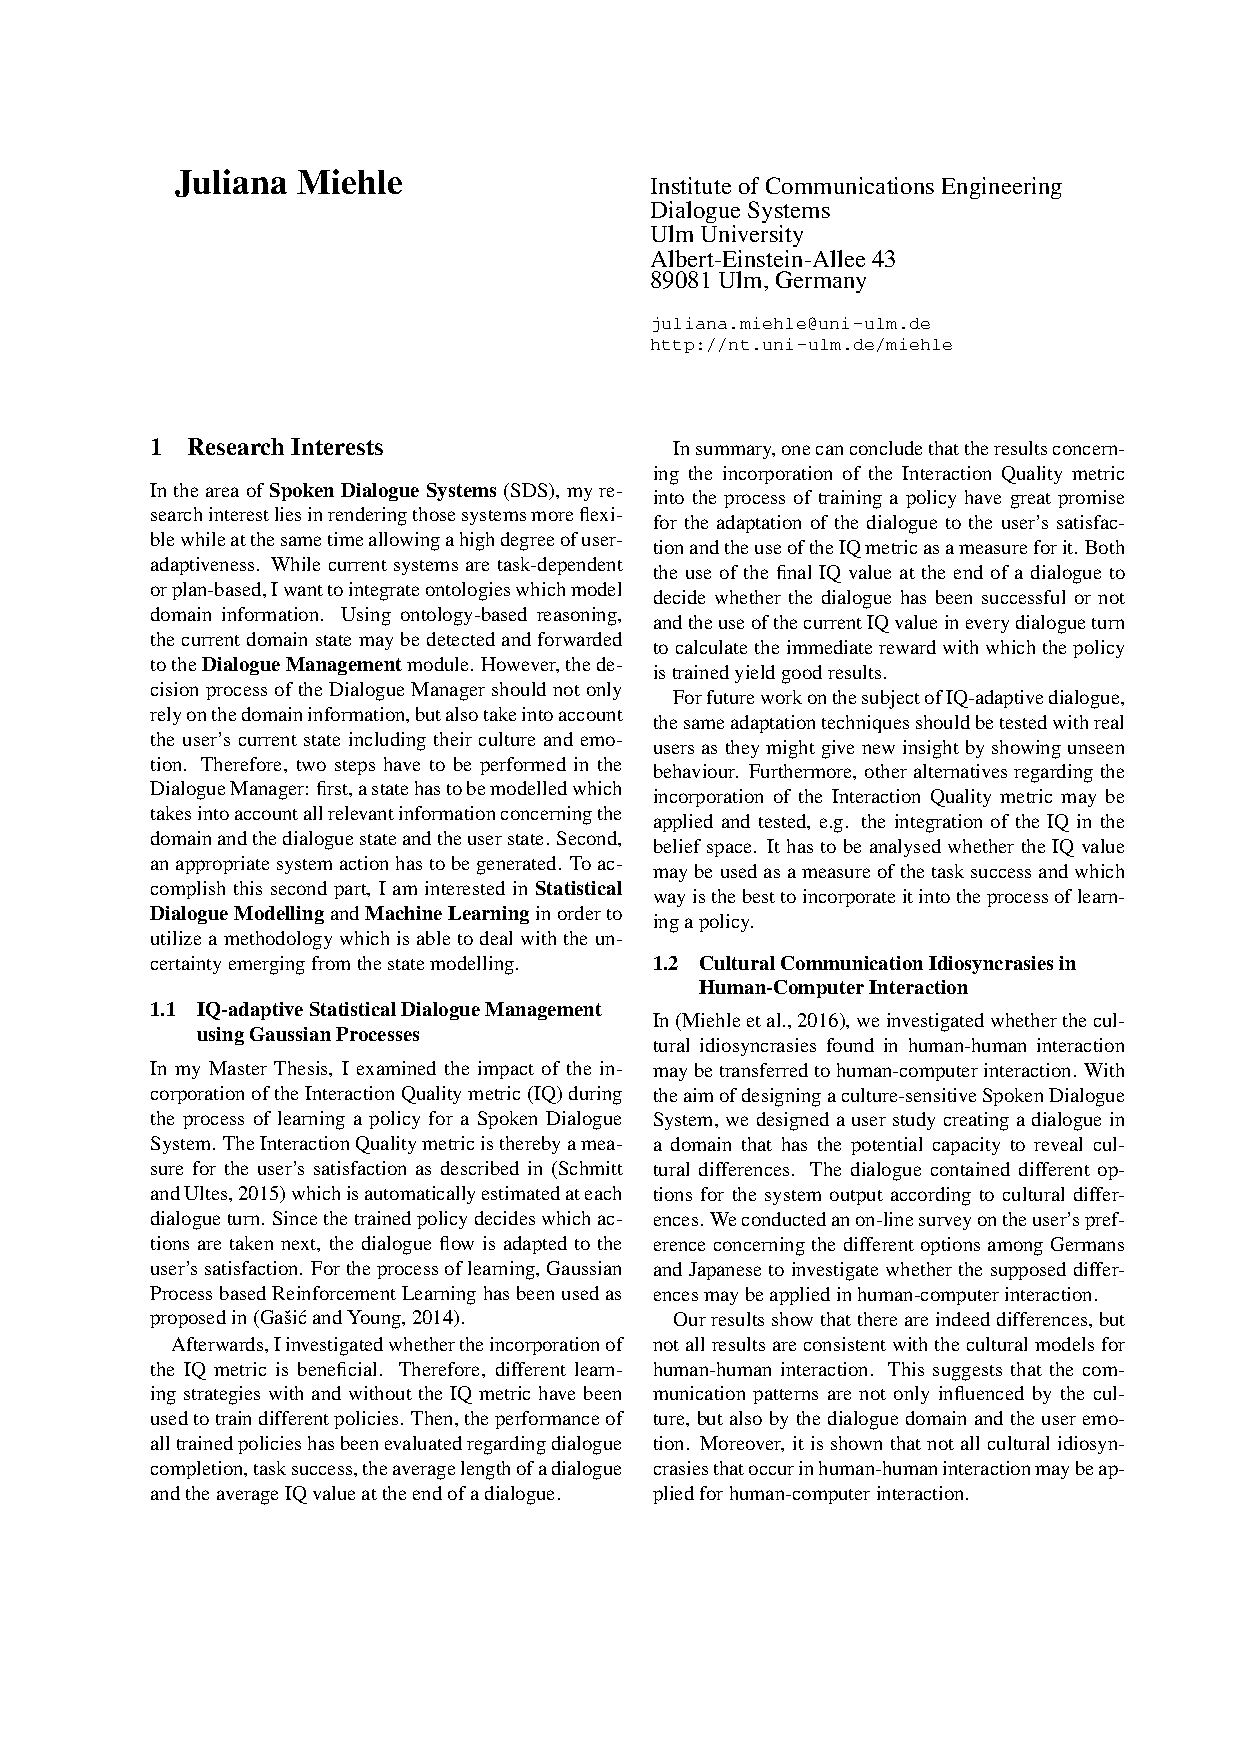
\includepdf[pages=-,pagecommand={}]{YRRSDS_2016_paper_4_juliana_miehle.pdf}
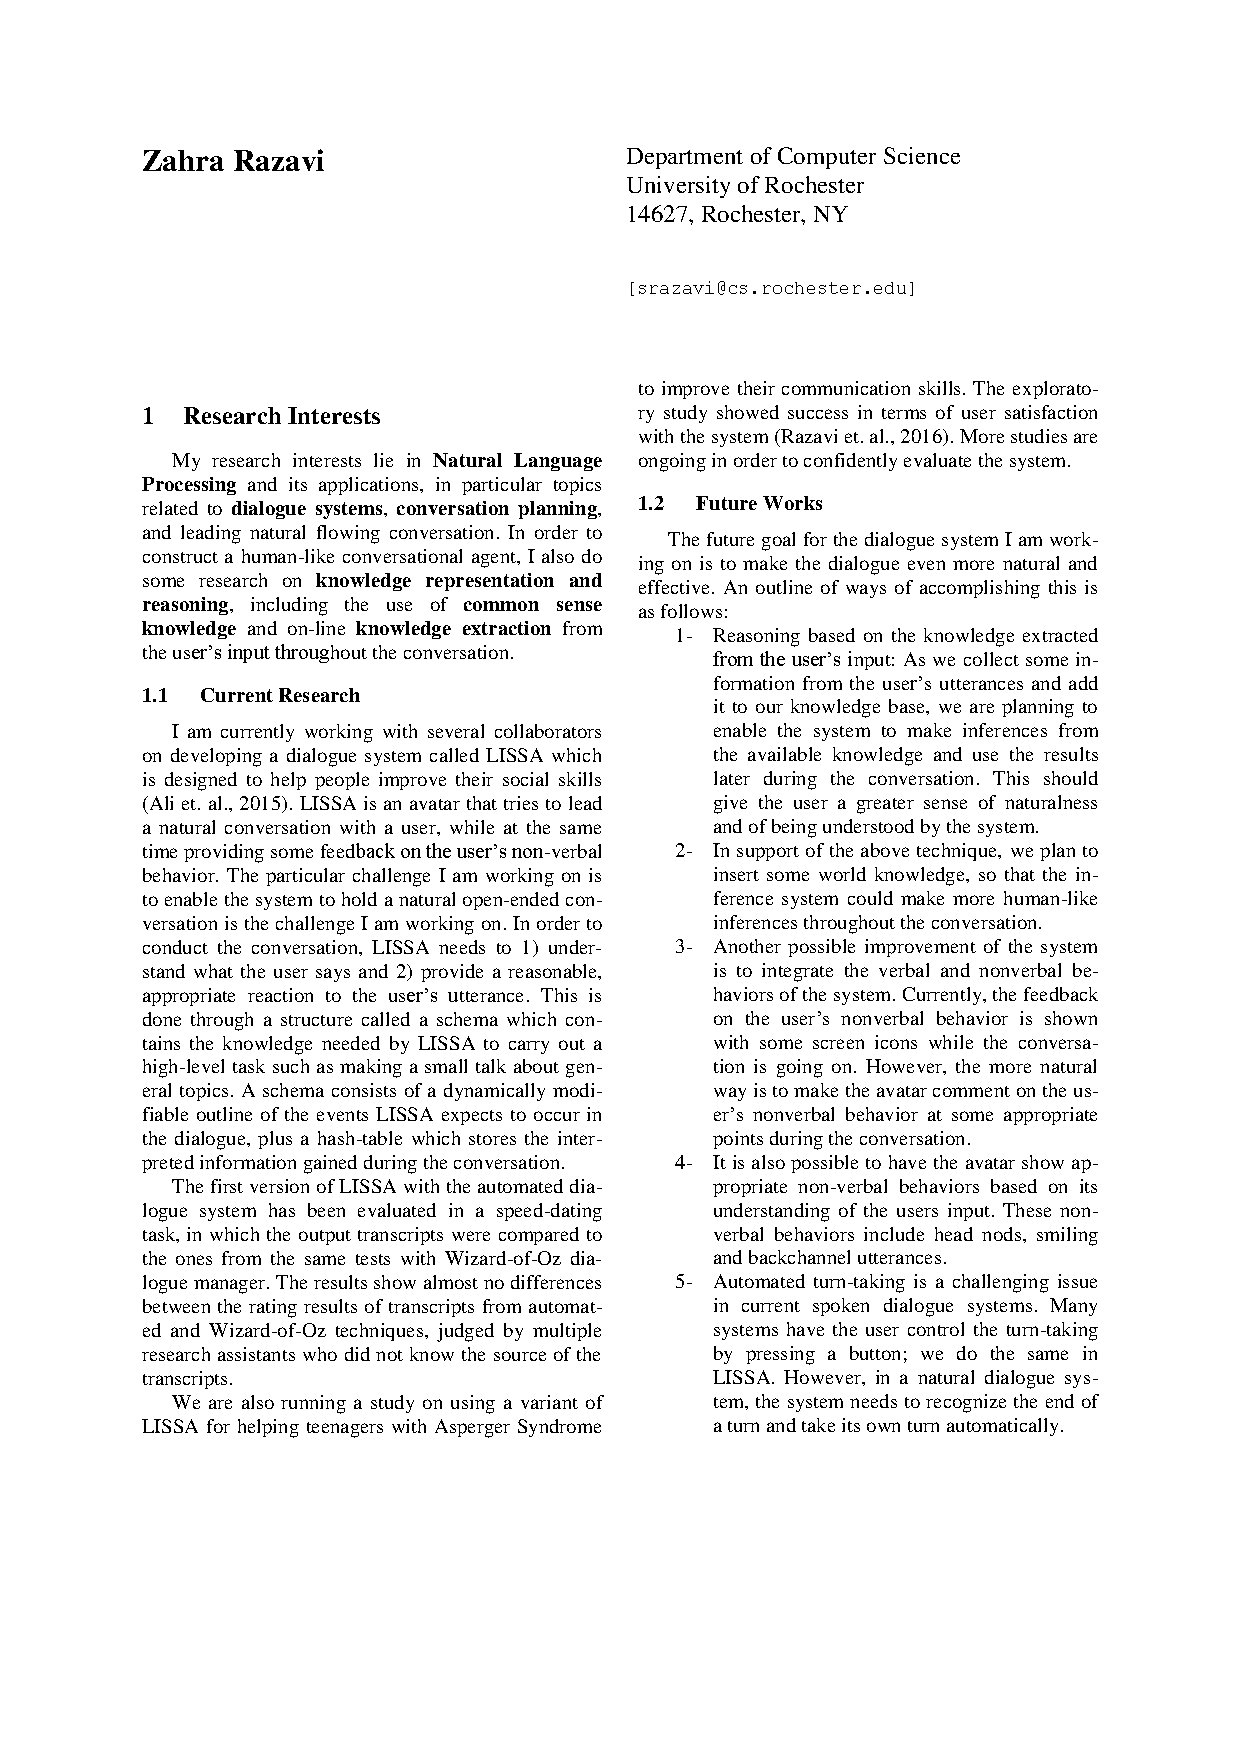
\includepdf[pages=-,pagecommand={}]{YRRSDS_2016_paper_5_zahra_razavi.pdf}
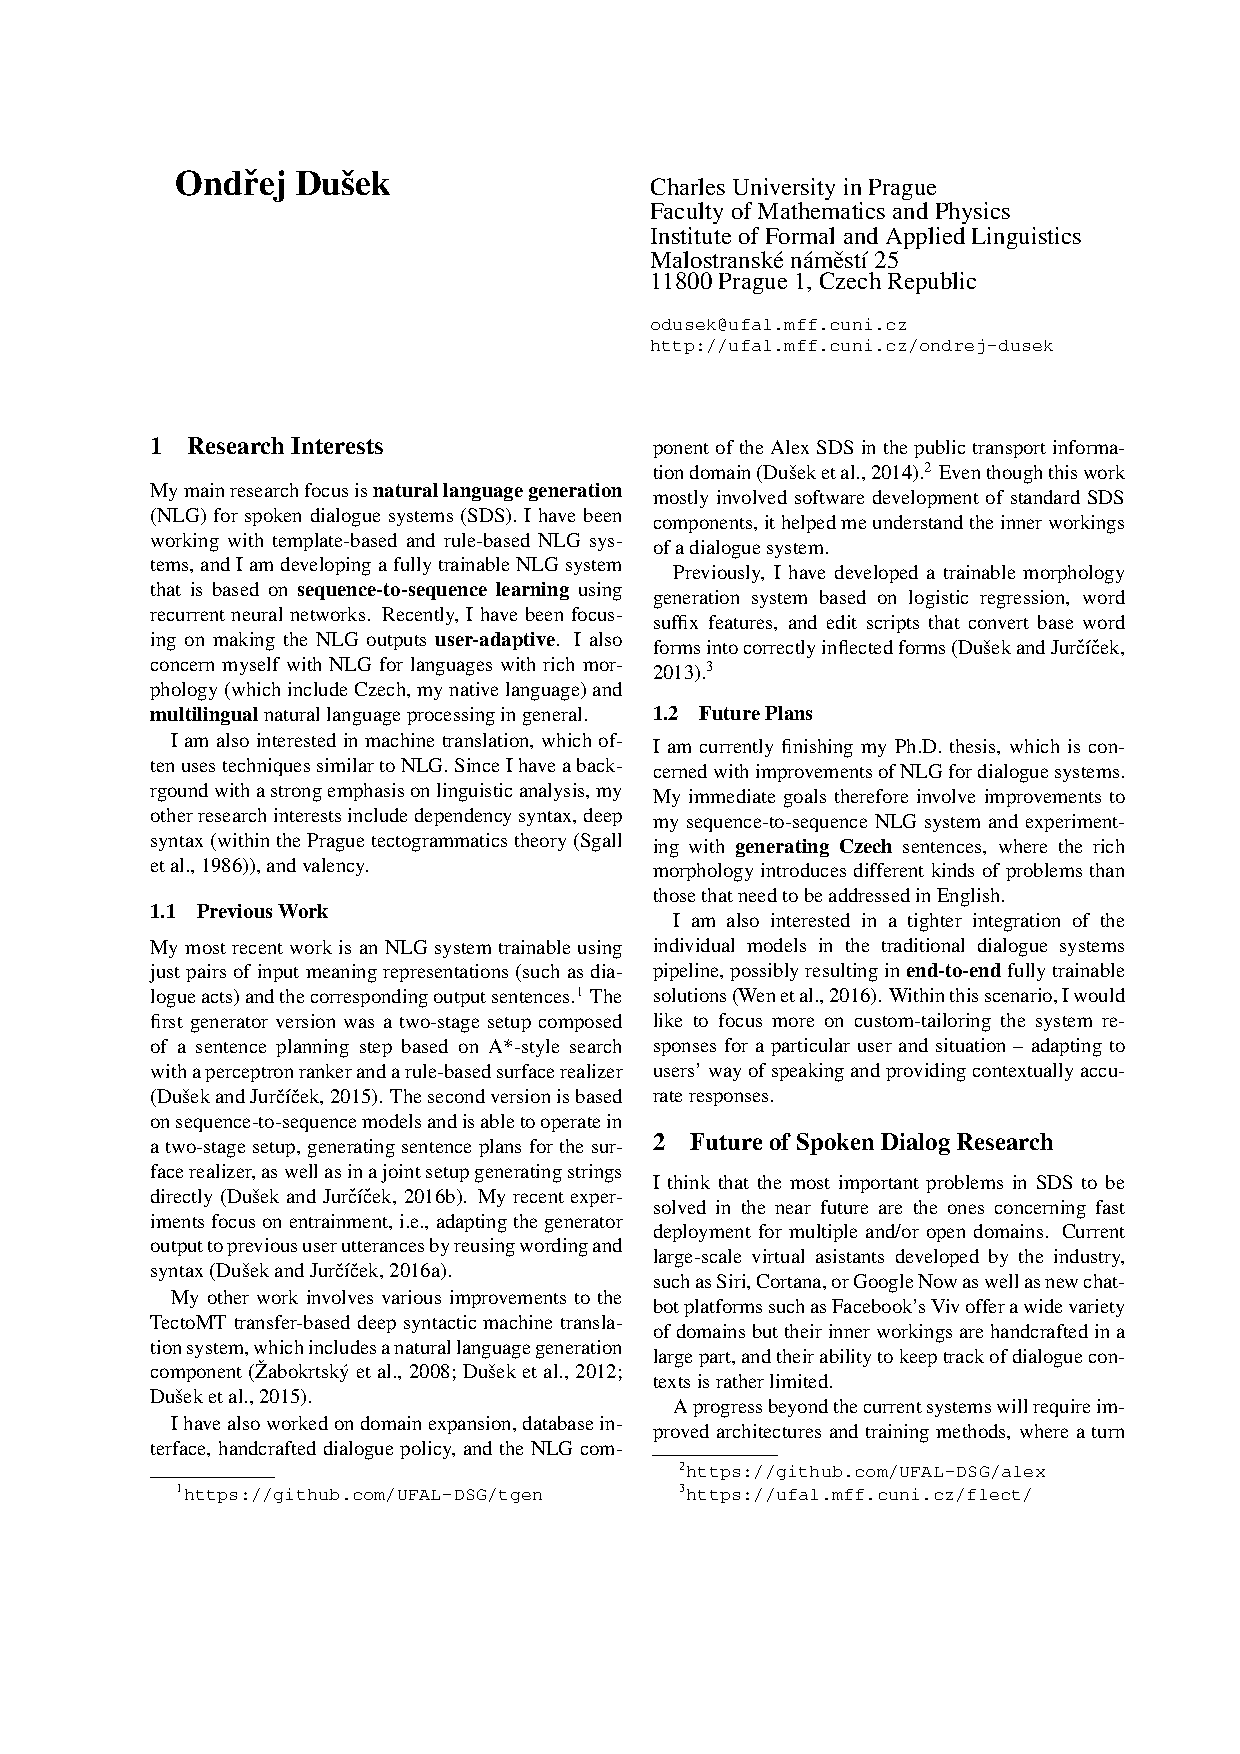
\includepdf[pages=-,pagecommand={}]{YRRSDS_2016_paper_6_ondrej_dusek.pdf}
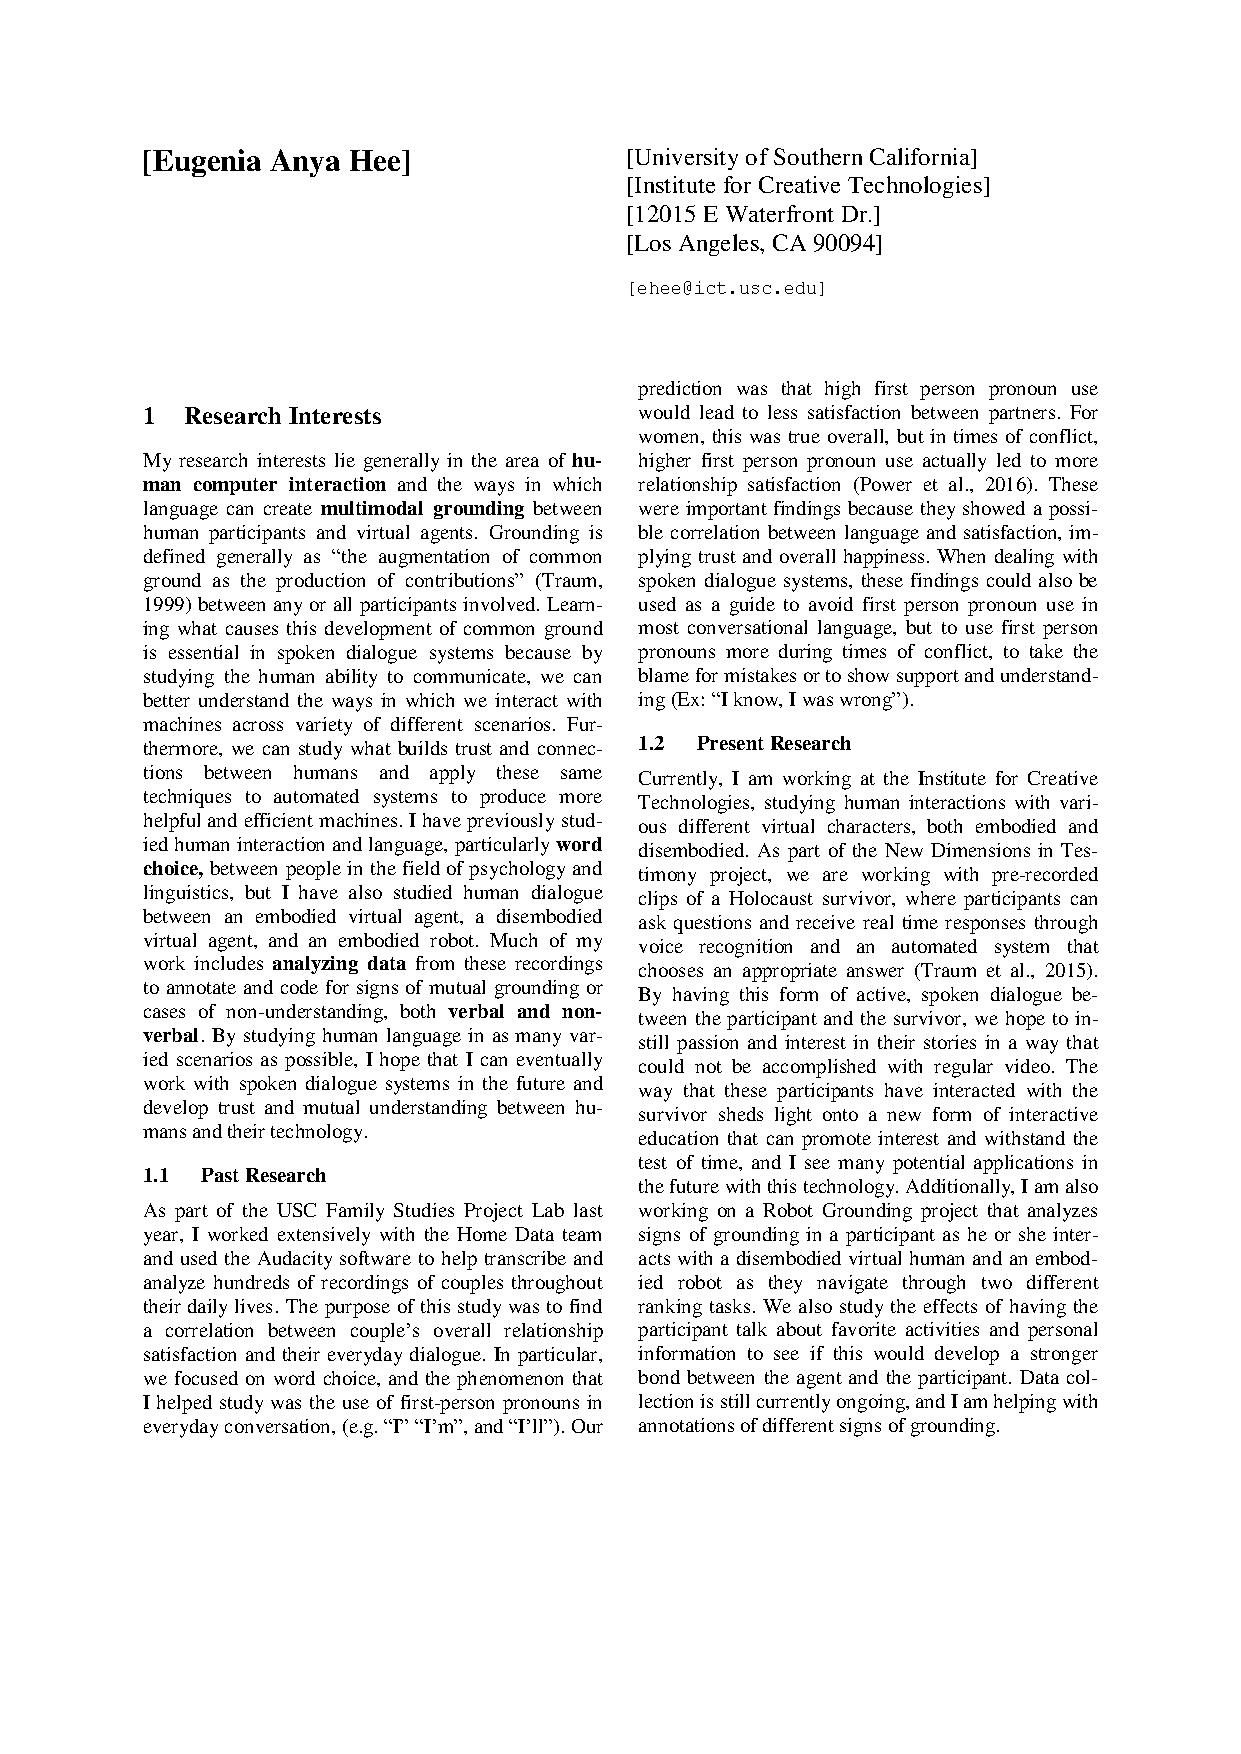
\includepdf[pages=-,pagecommand={}]{YRRSDS_2016_paper_7_eugenia_hee.pdf}
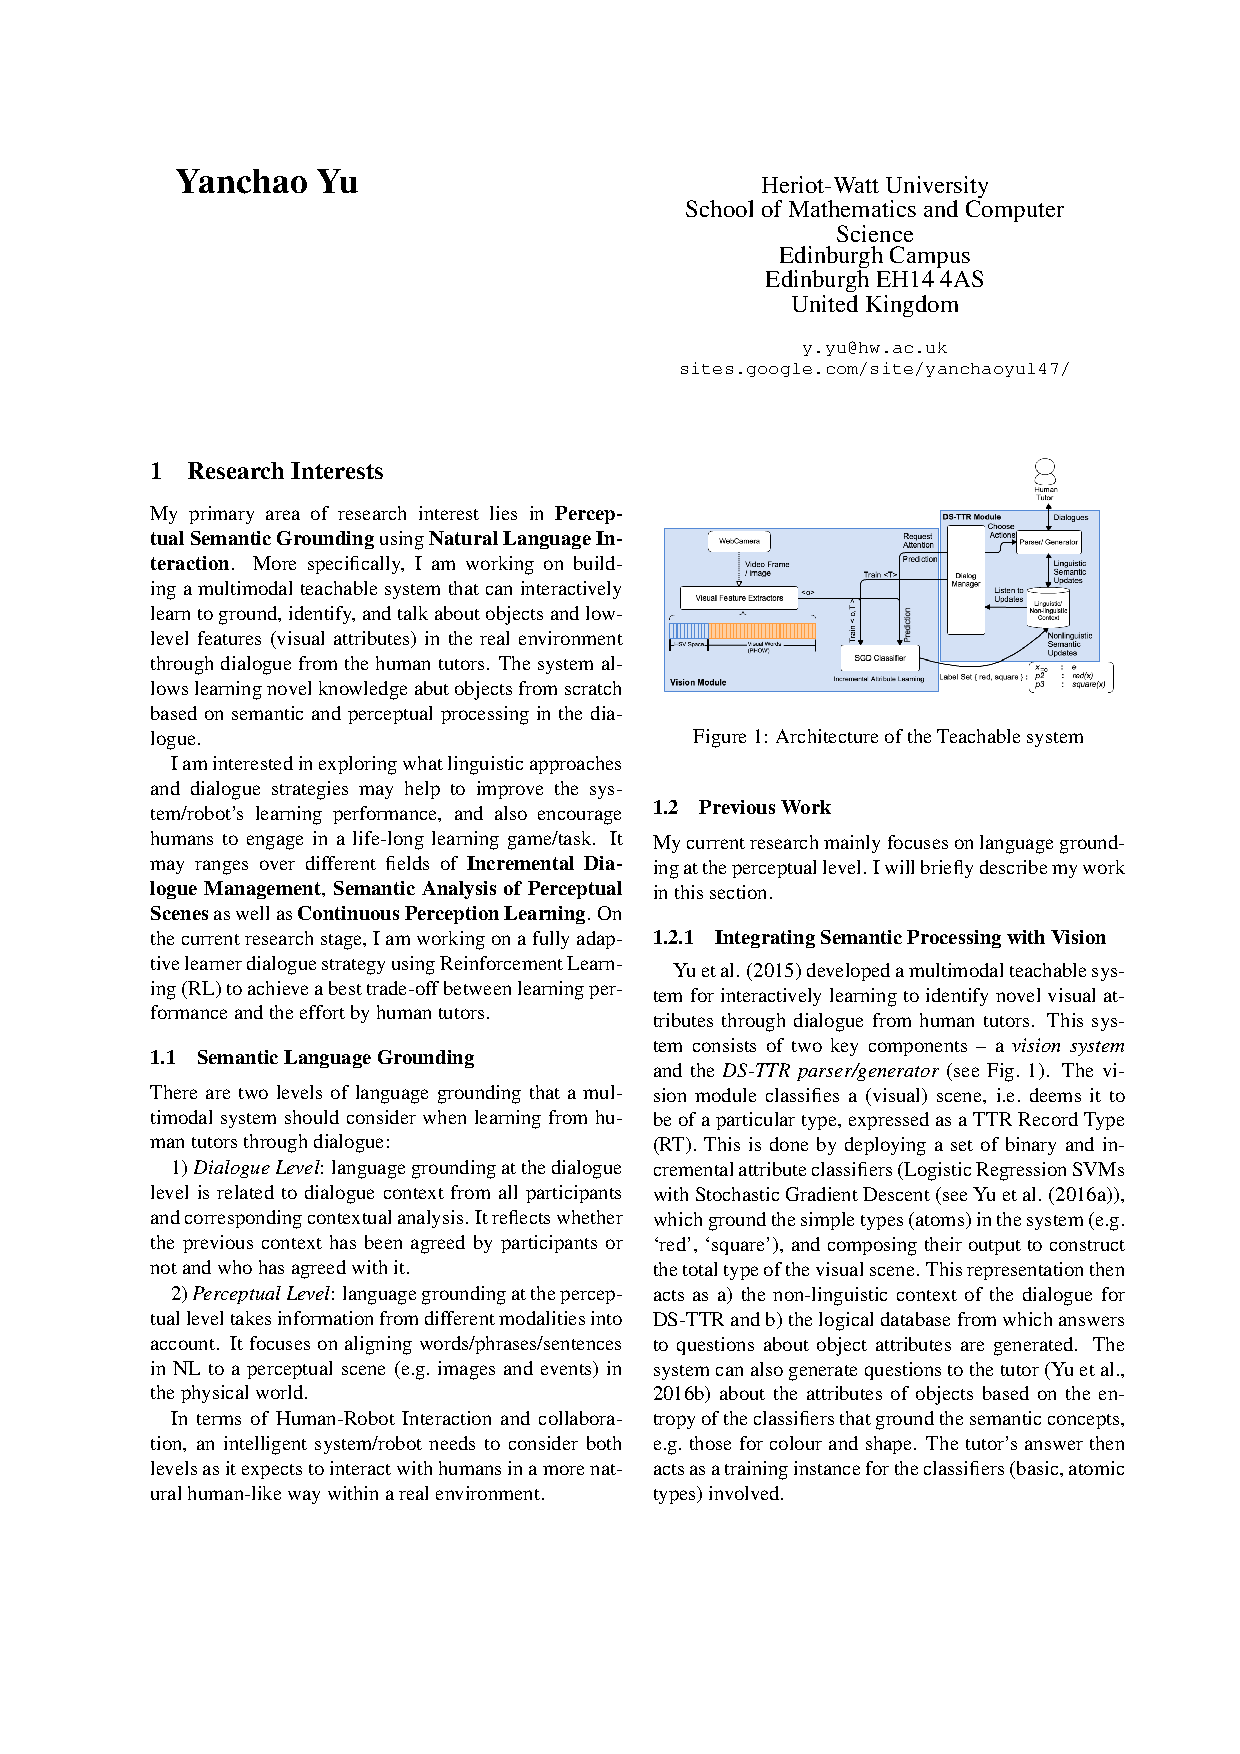
\includepdf[pages=-,pagecommand={}]{YRRSDS_2016_paper_8_uanchao_yu.pdf}
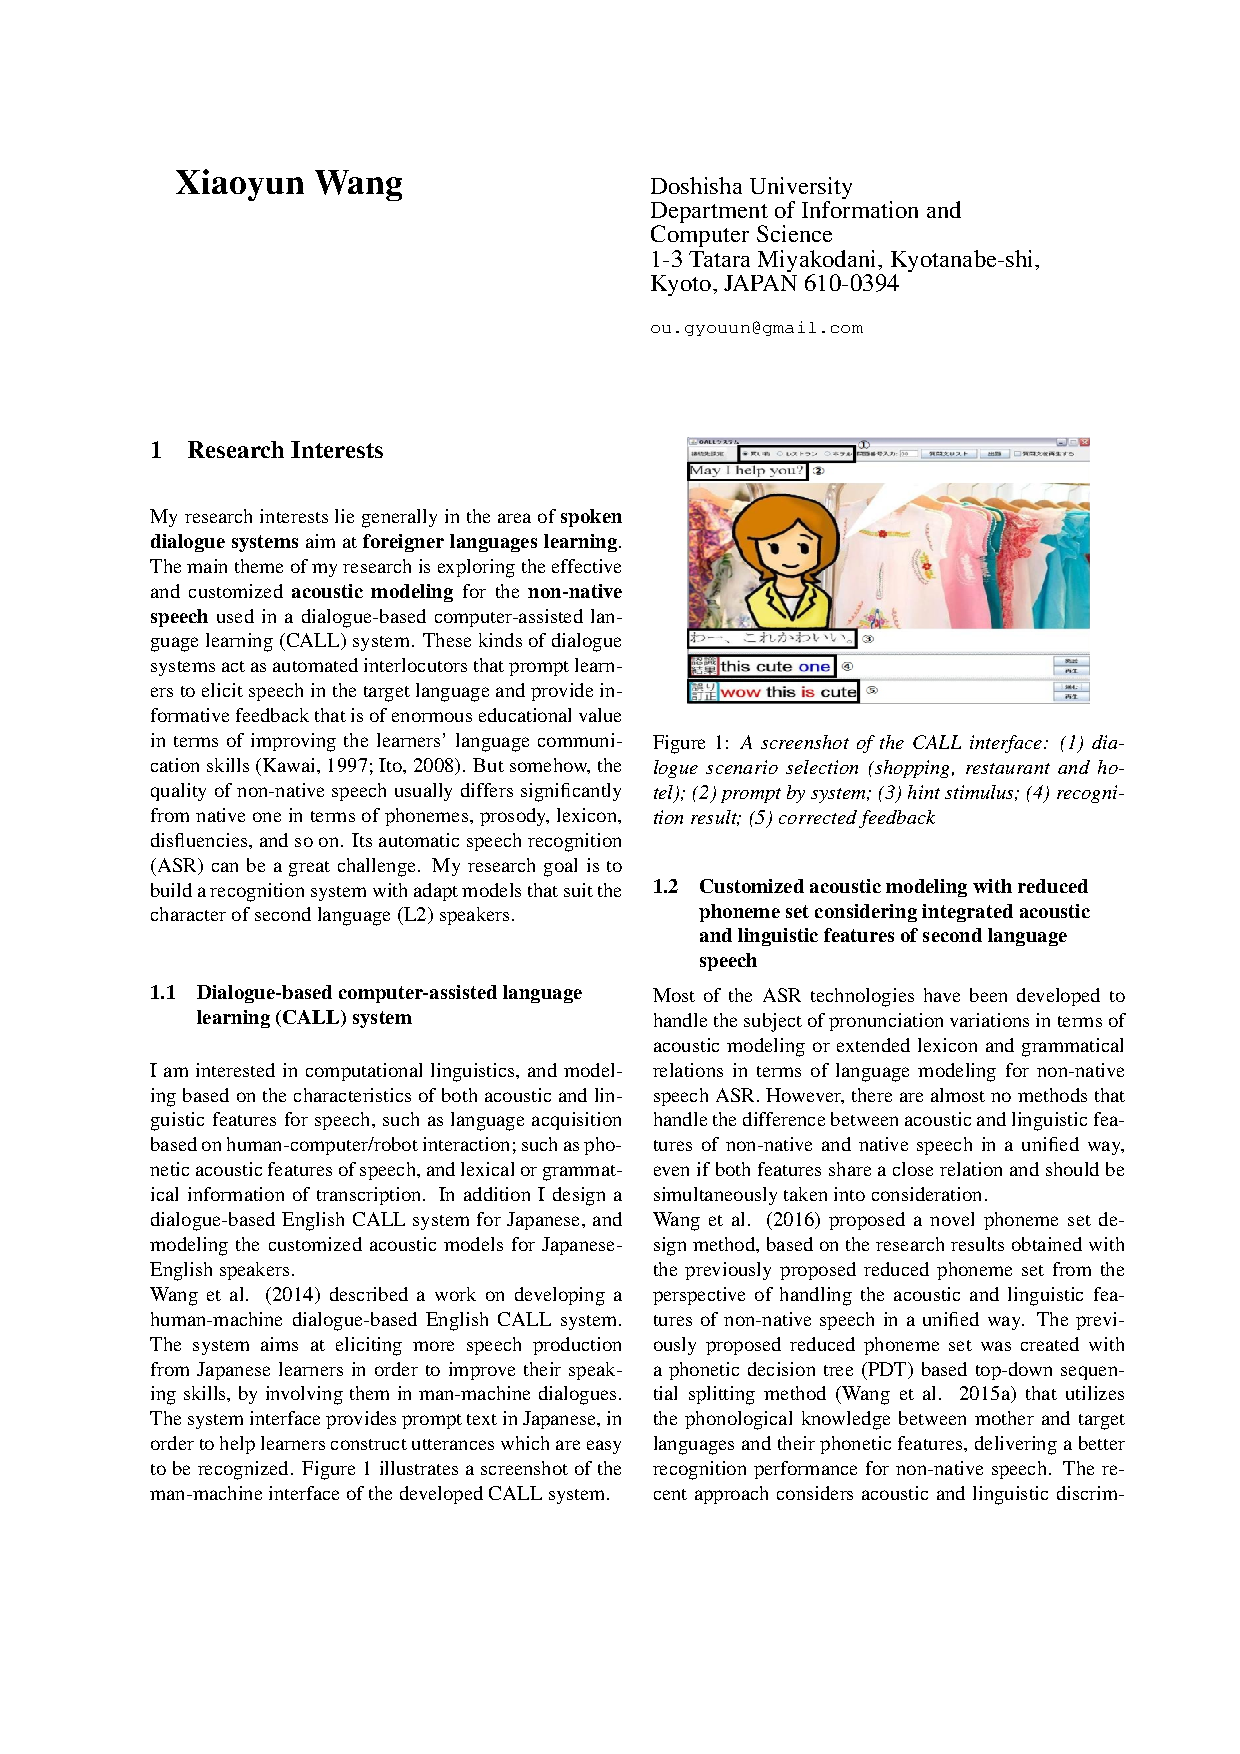
\includepdf[pages=-,pagecommand={}]{YRRSDS_2016_paper_9_xiaoyun_wang.pdf}
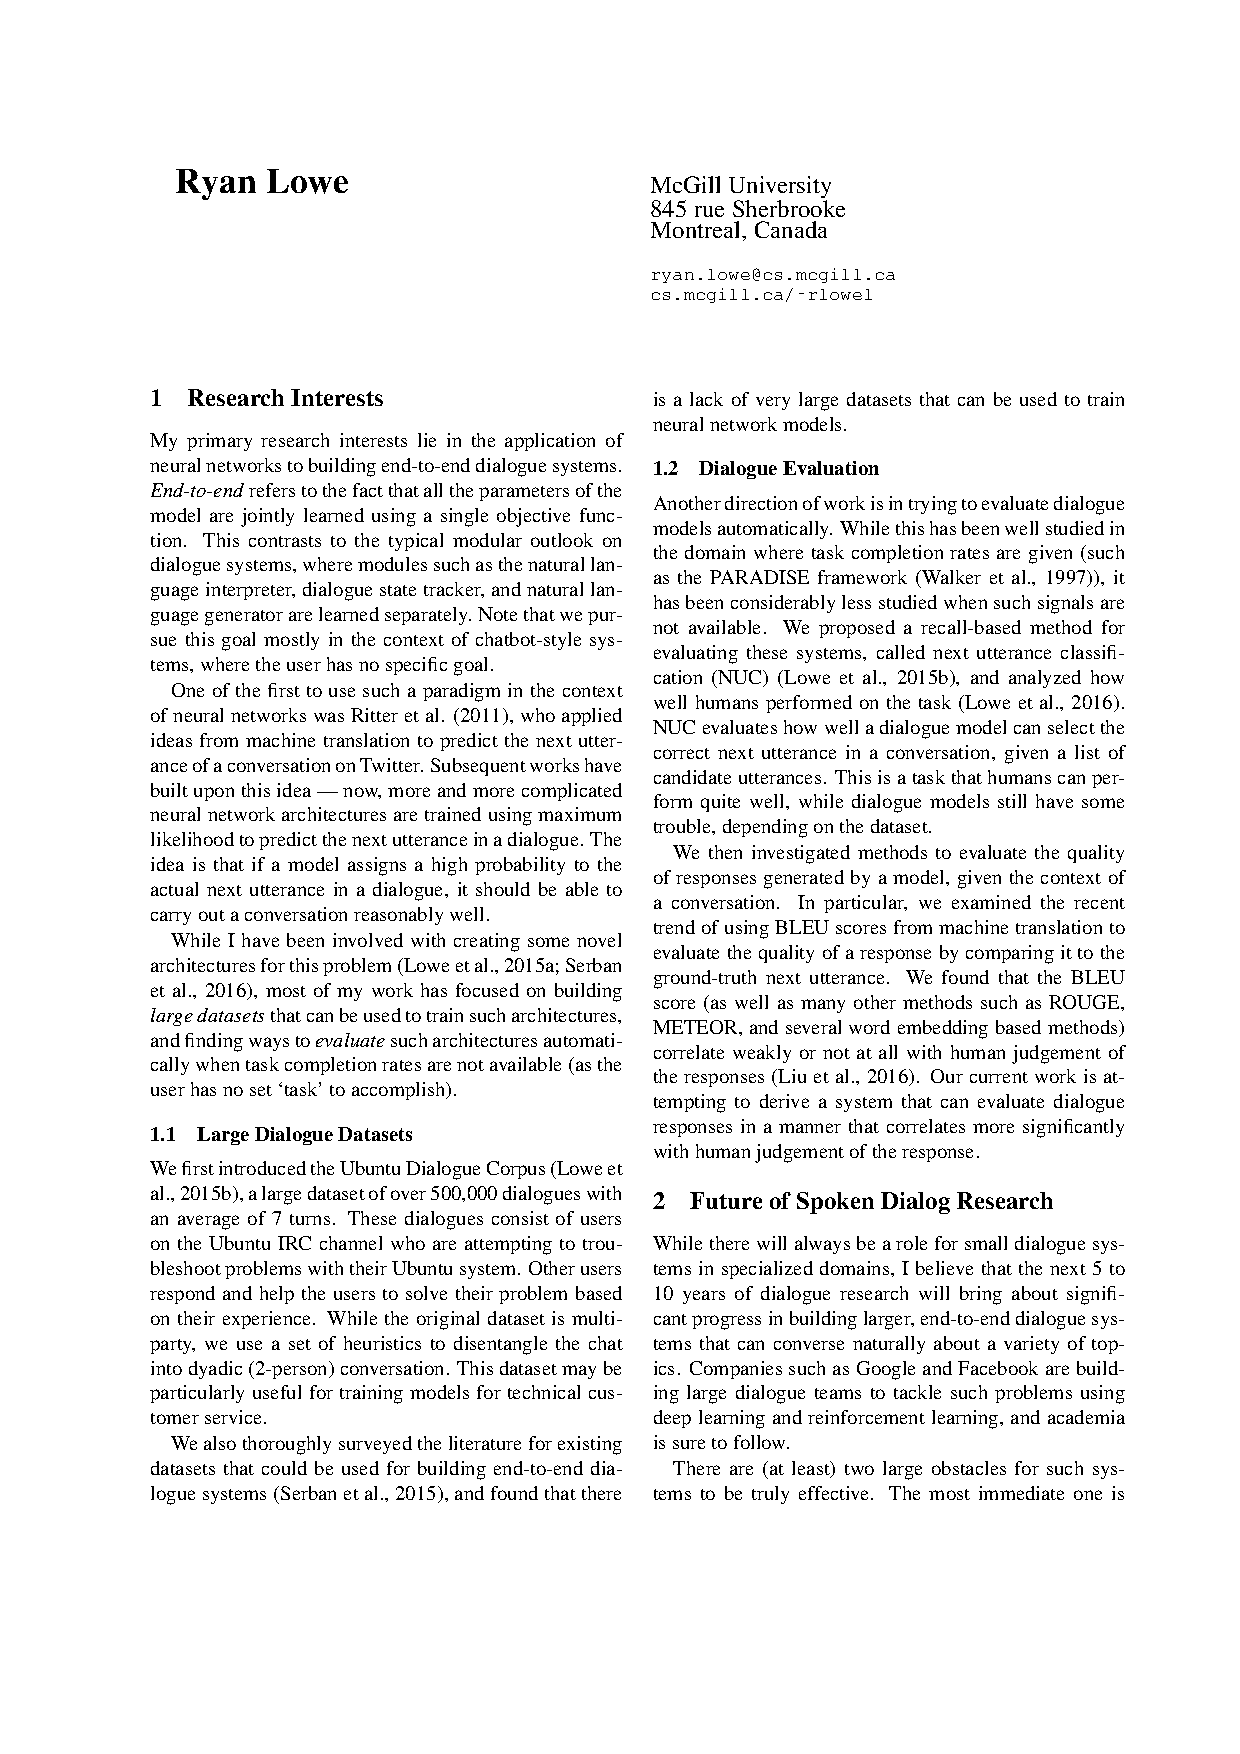
\includepdf[pages=-,pagecommand={}]{YRRSDS_2016_paper_10_rayn_lowe.pdf}
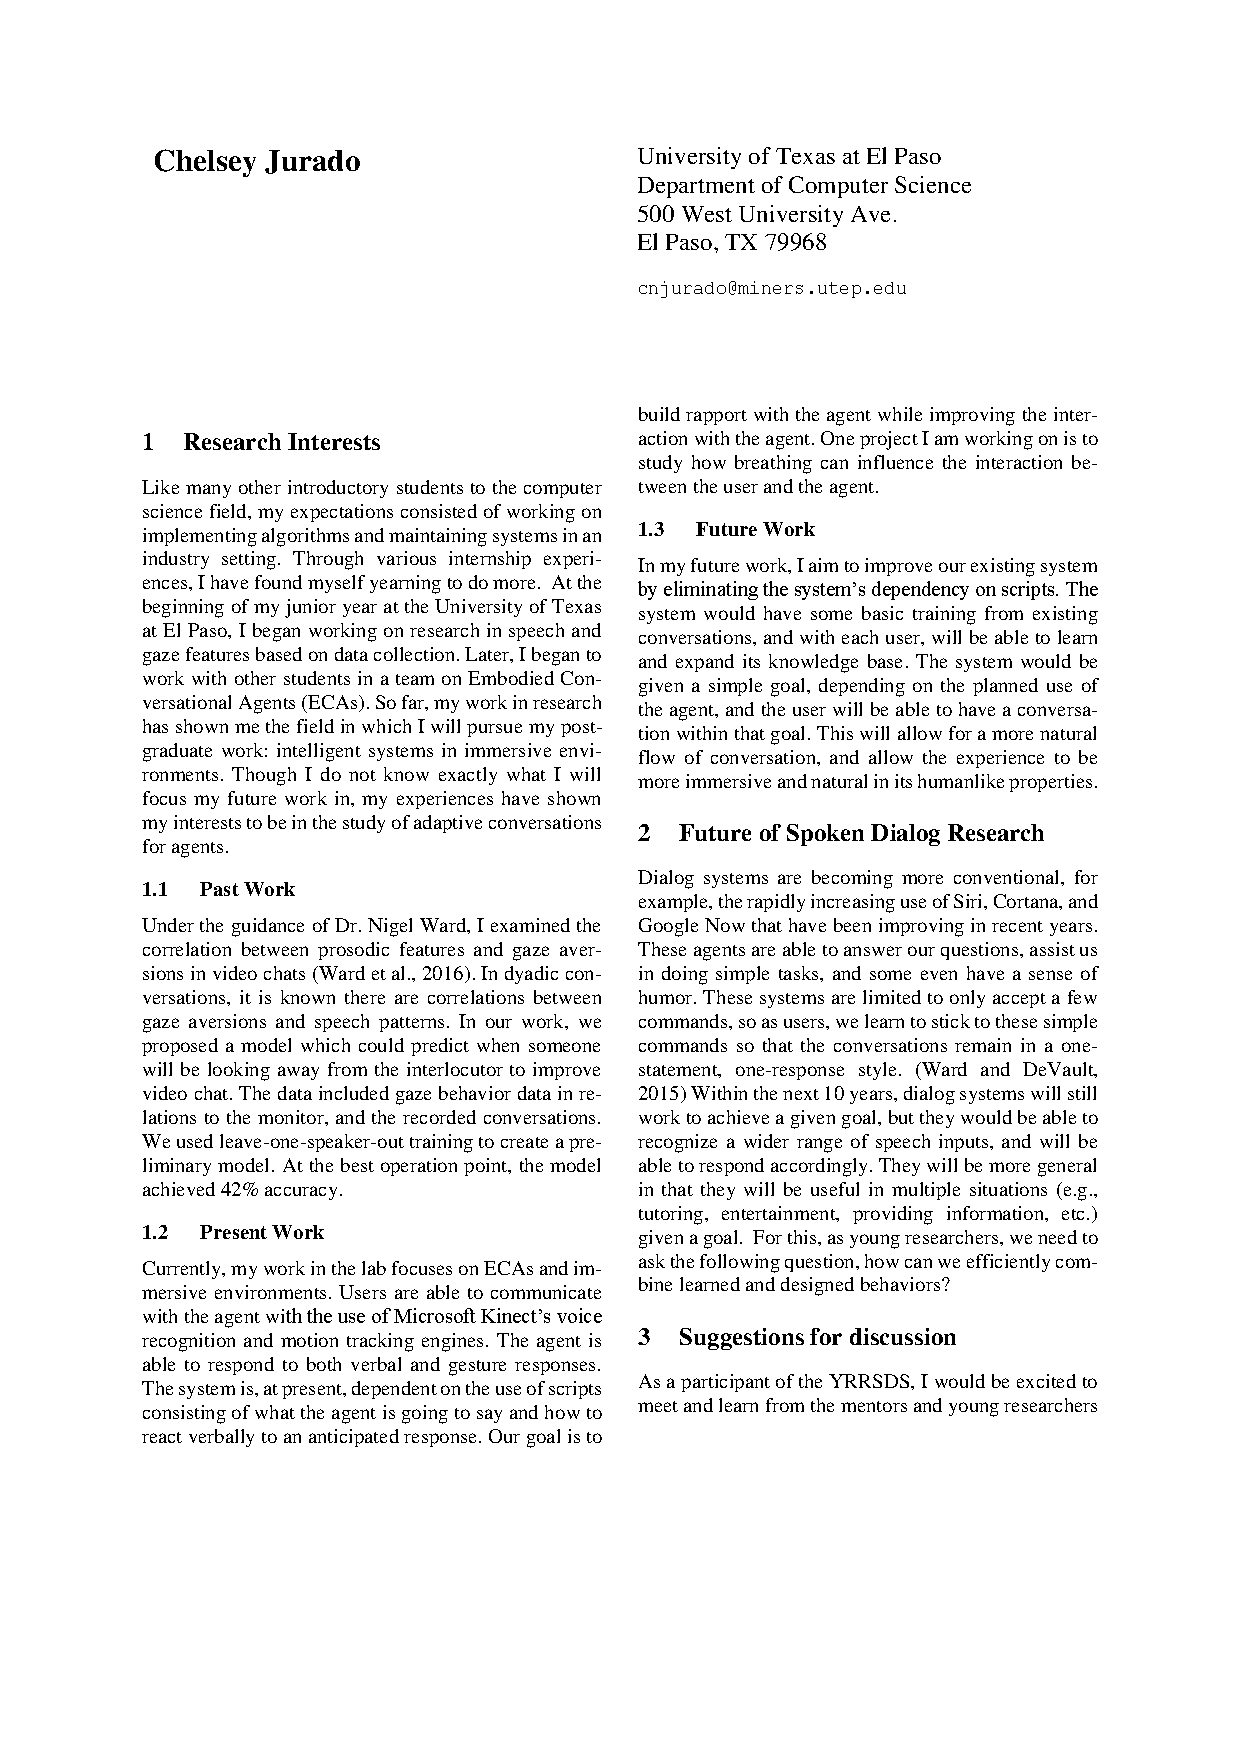
\includepdf[pages=-,pagecommand={}]{YRRSDS_2016_paper_11_chelsey_jurado.pdf}
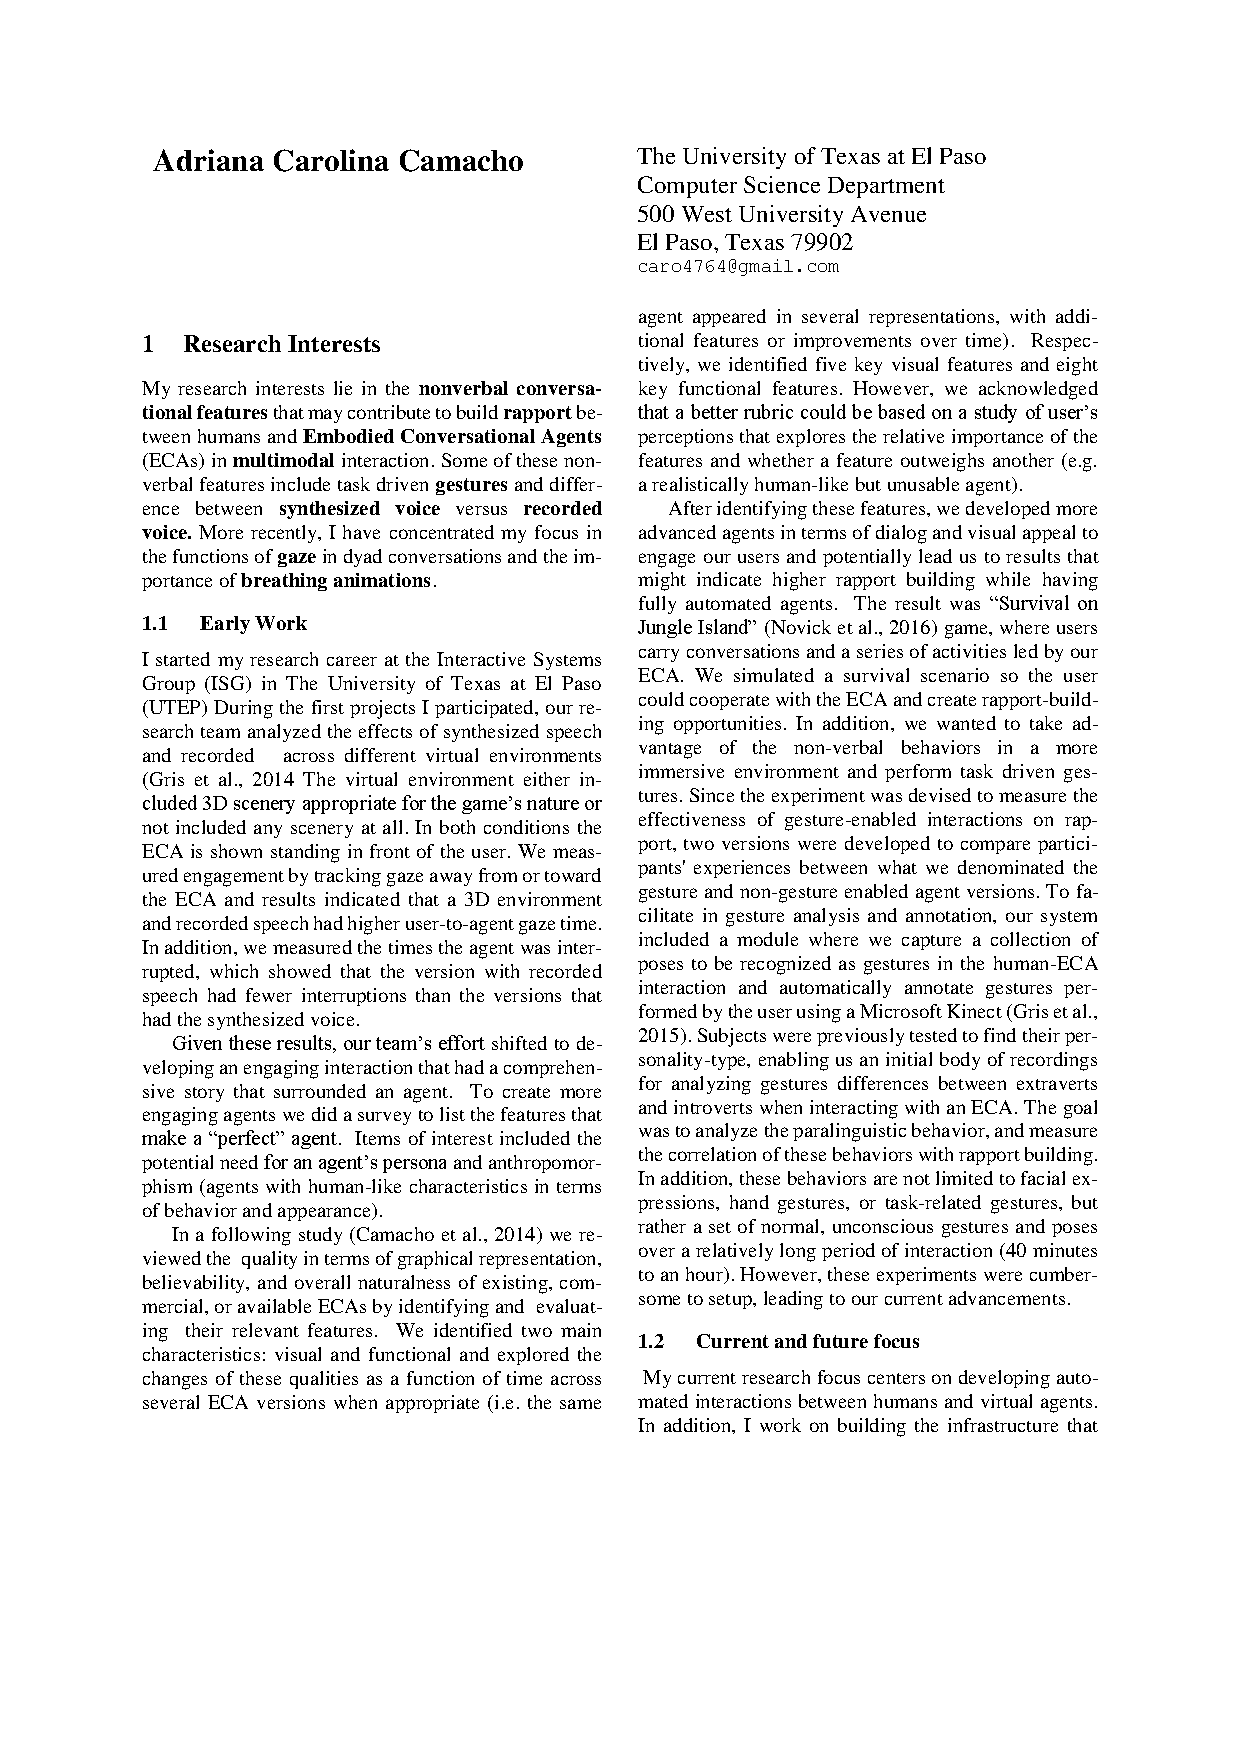
\includepdf[pages=-,pagecommand={}]{YRRSDS_2016_paper_12_adriana_camacho.pdf}
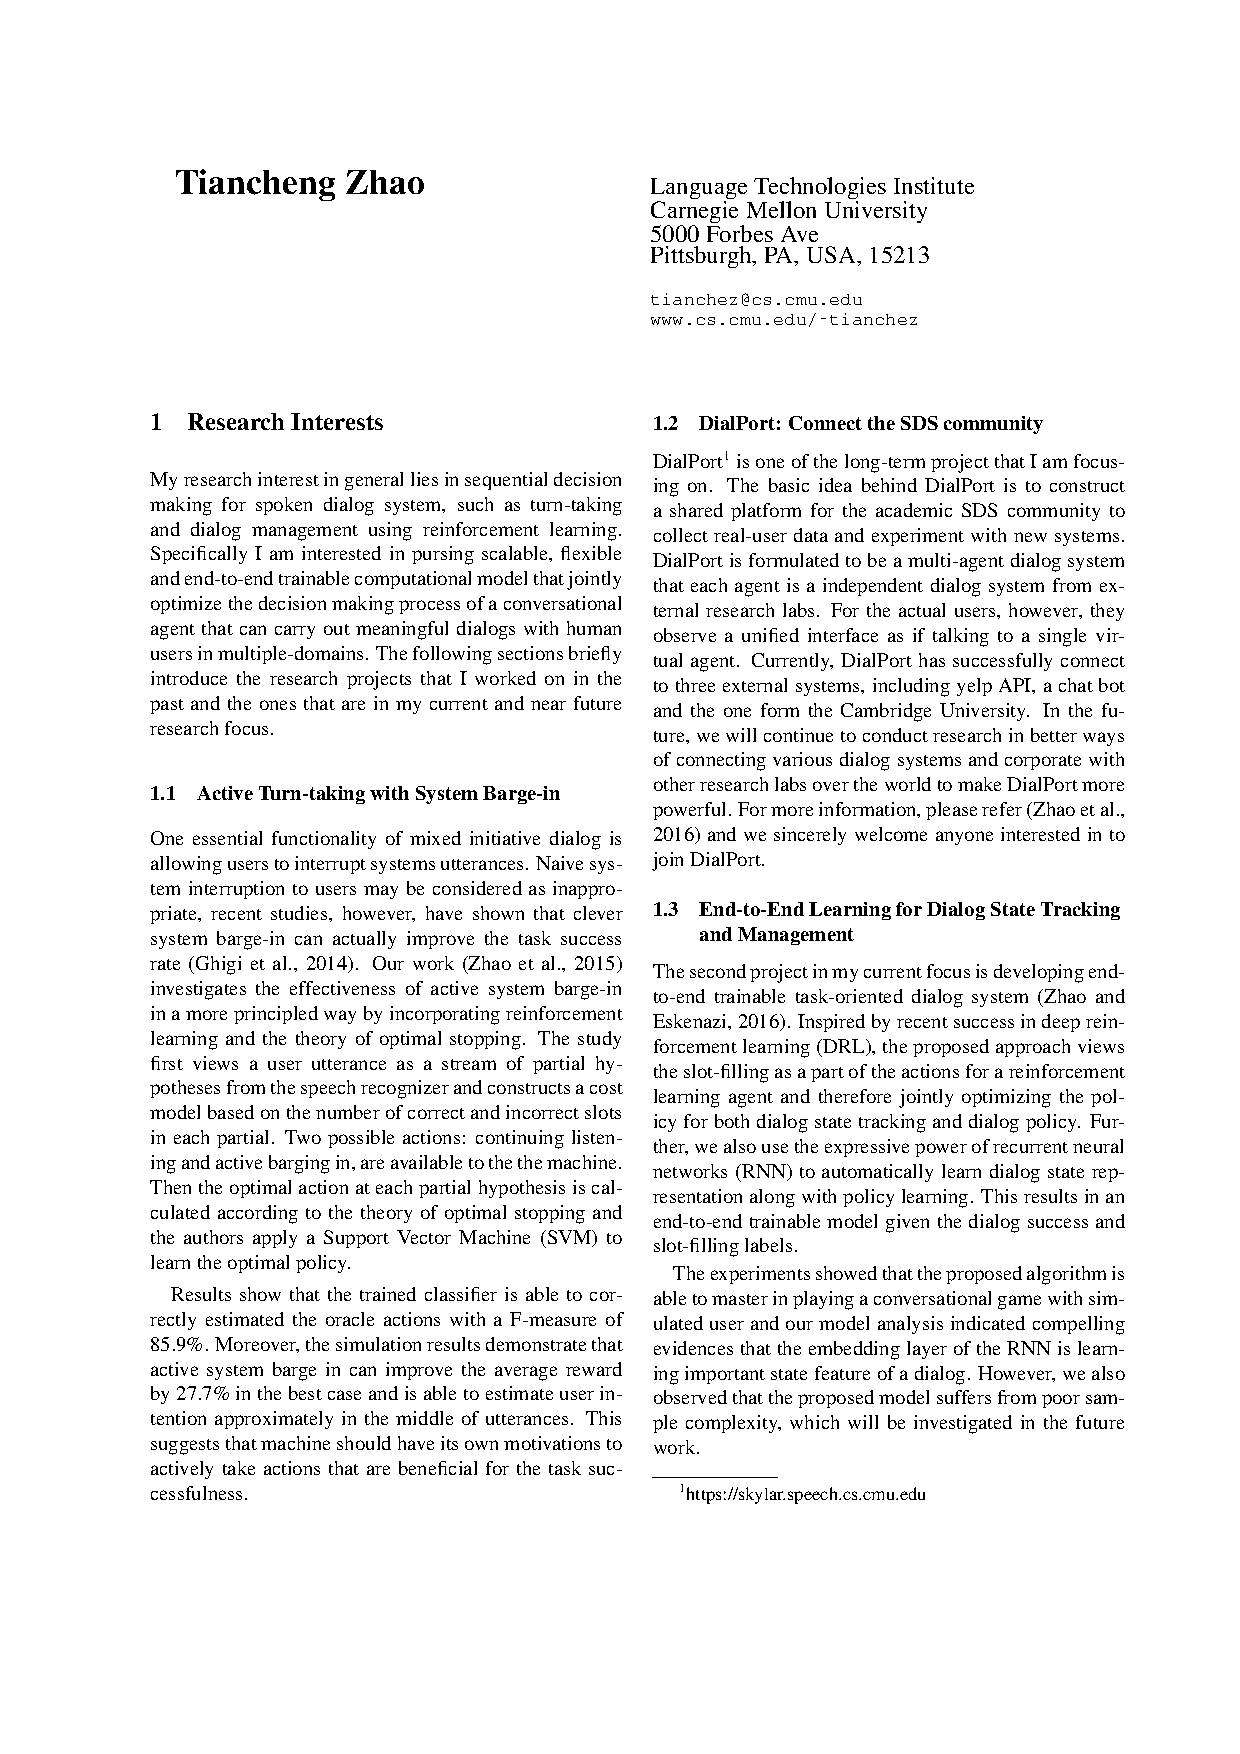
\includepdf[pages=-,pagecommand={}]{YRRSDS_2016_paper_14_tiancheng_zhao.pdf}
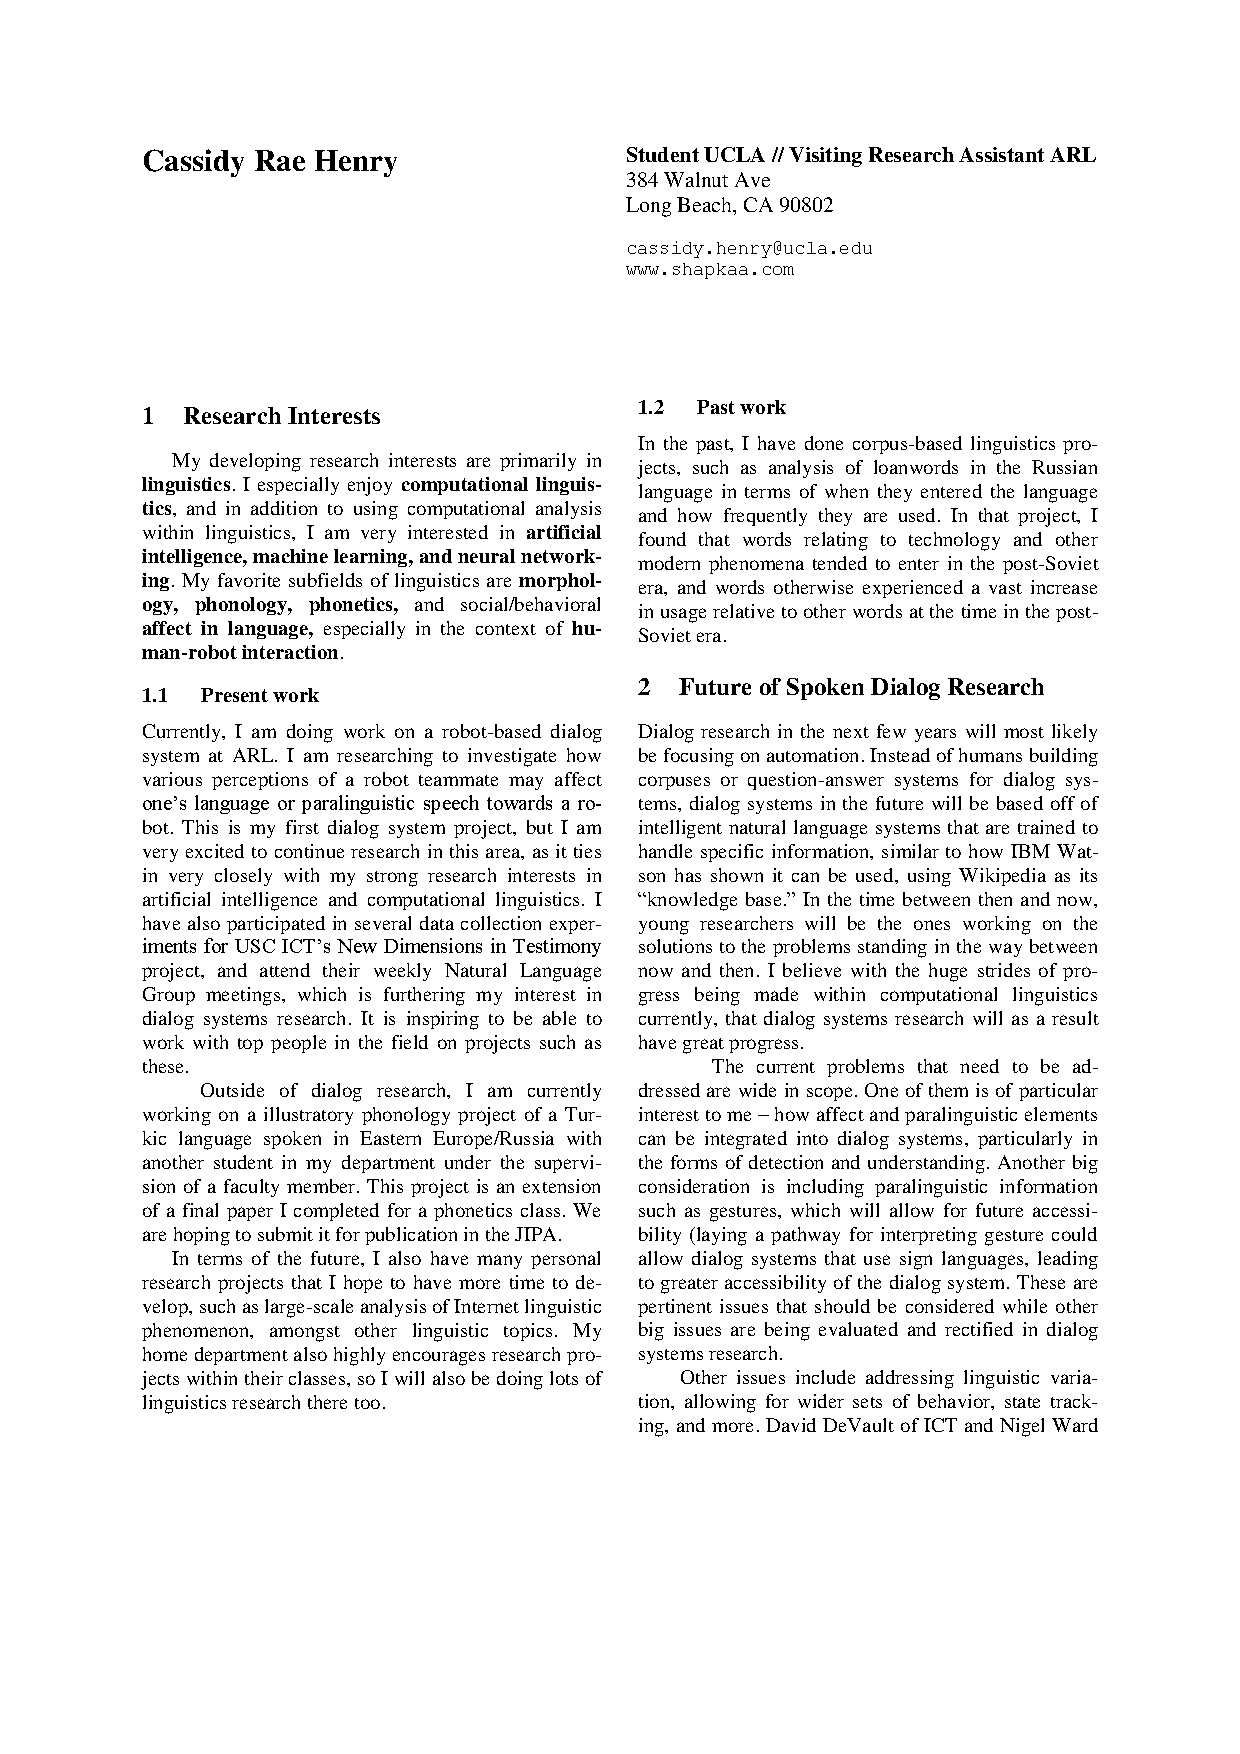
\includepdf[pages=-,pagecommand={}]{YRRSDS_2016_paper_15_cassidy_henry.pdf}
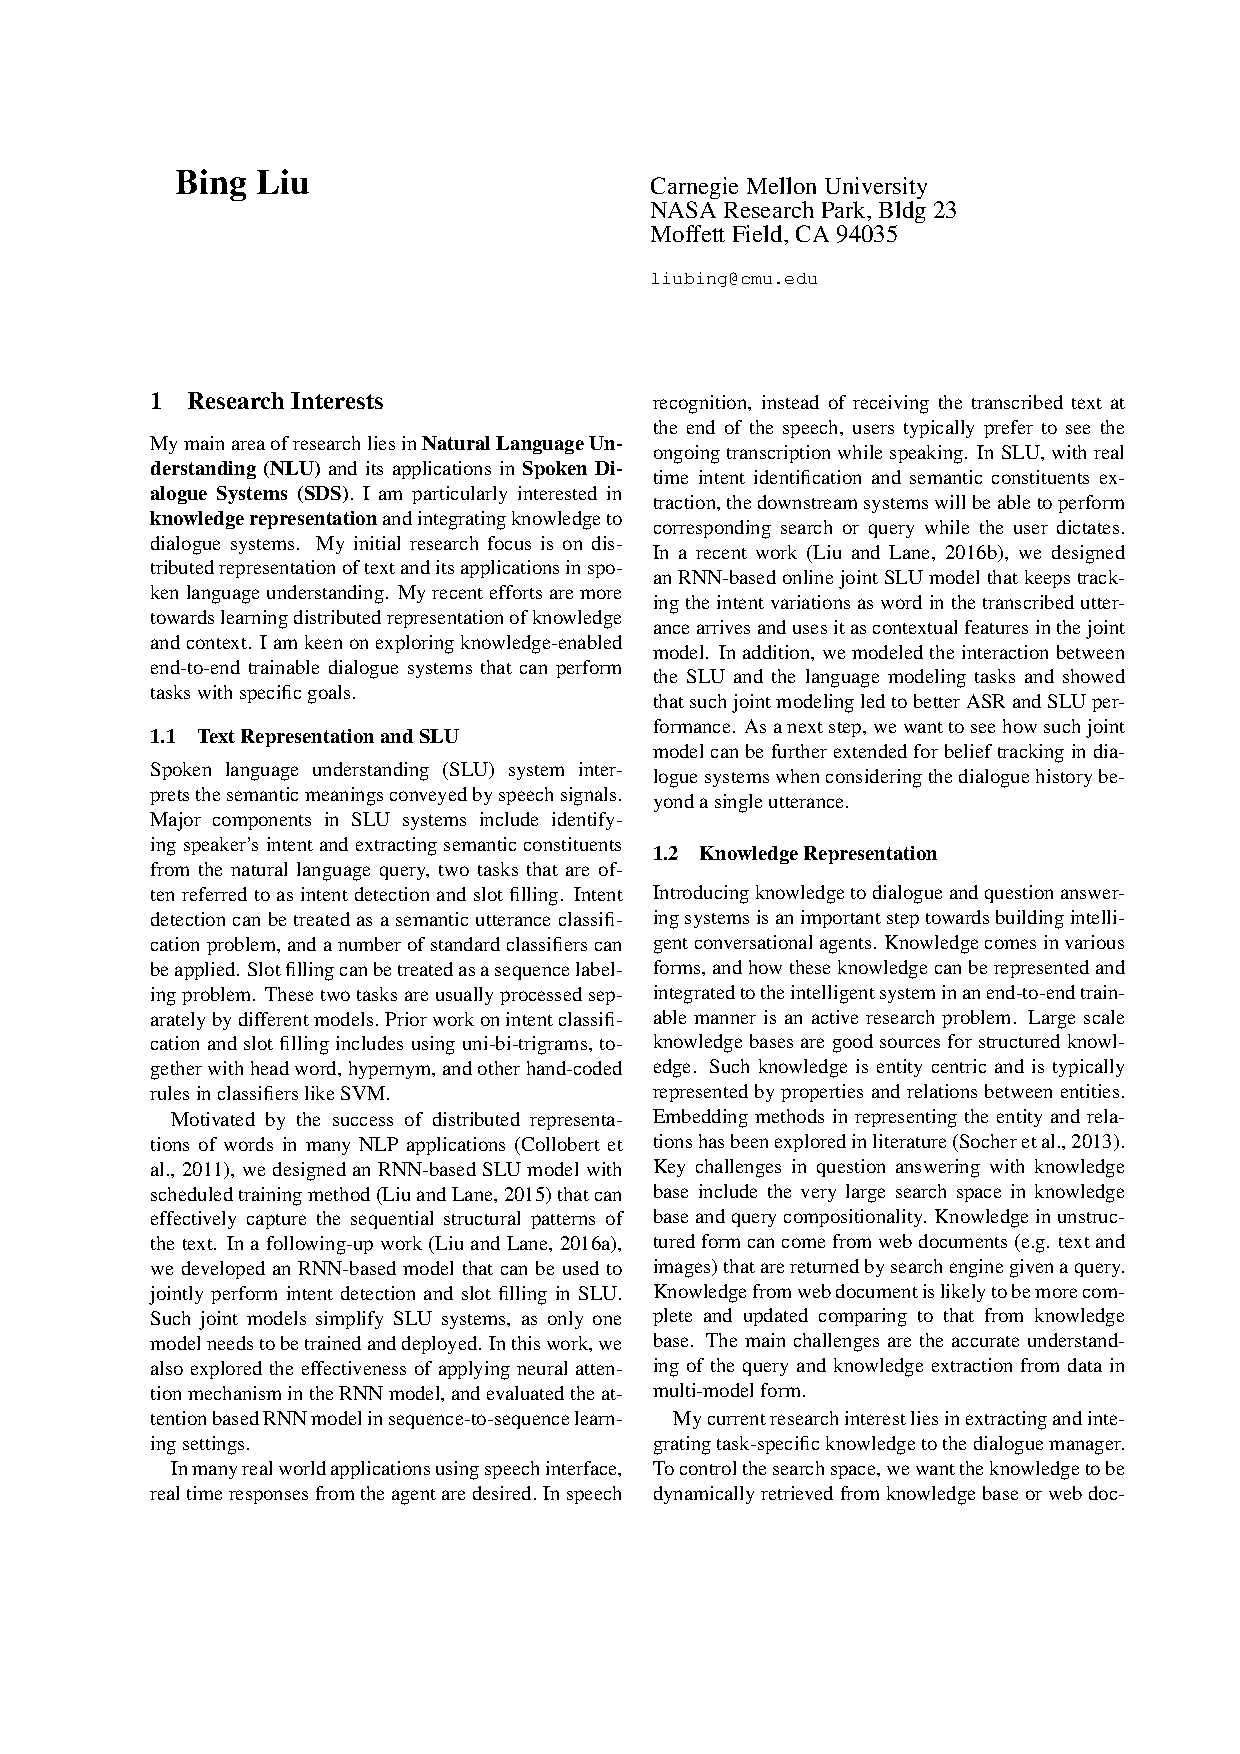
\includepdf[pages=-,pagecommand={}]{YRRSDS_2016_paper_16_bing_liu.pdf}
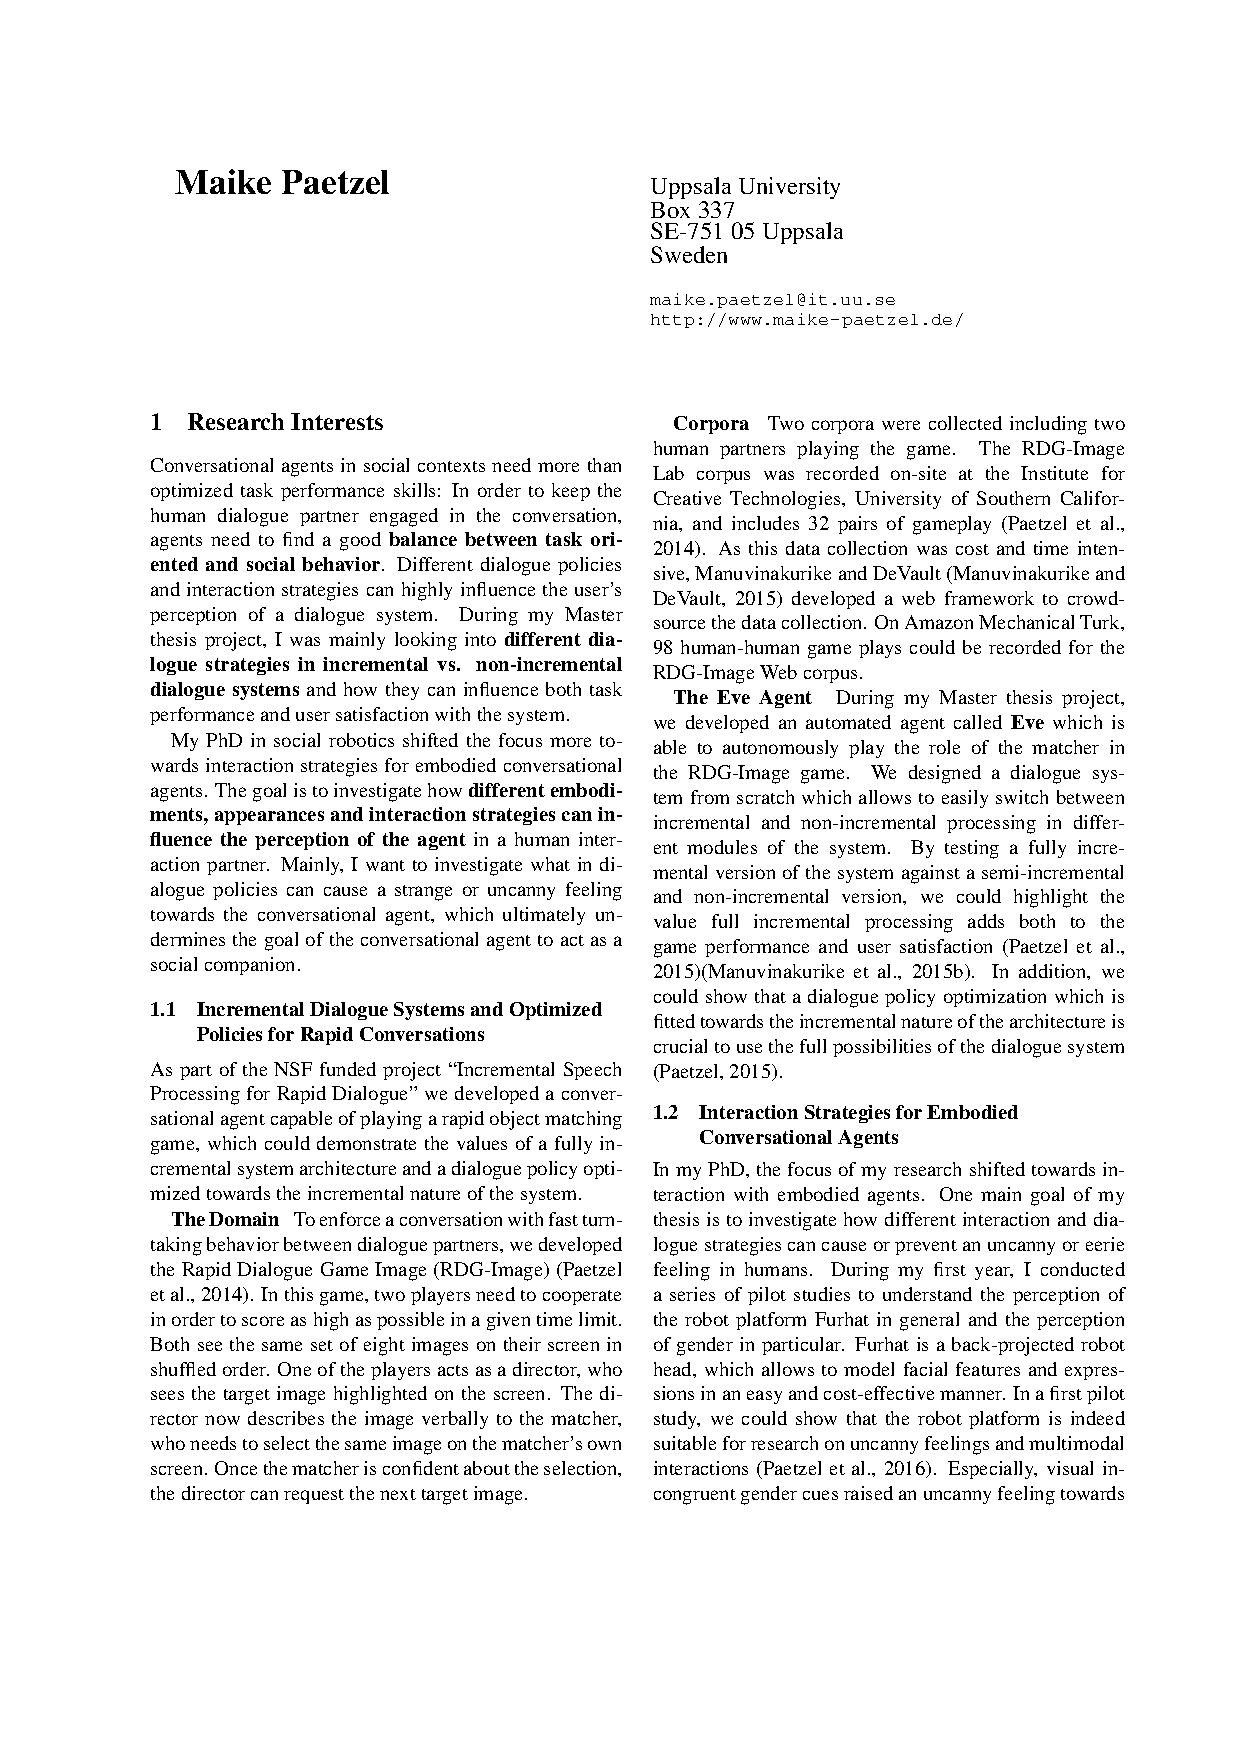
\includepdf[pages=-,pagecommand={}]{YRRSDS_2016_paper_17_maike_paetzel.pdf}
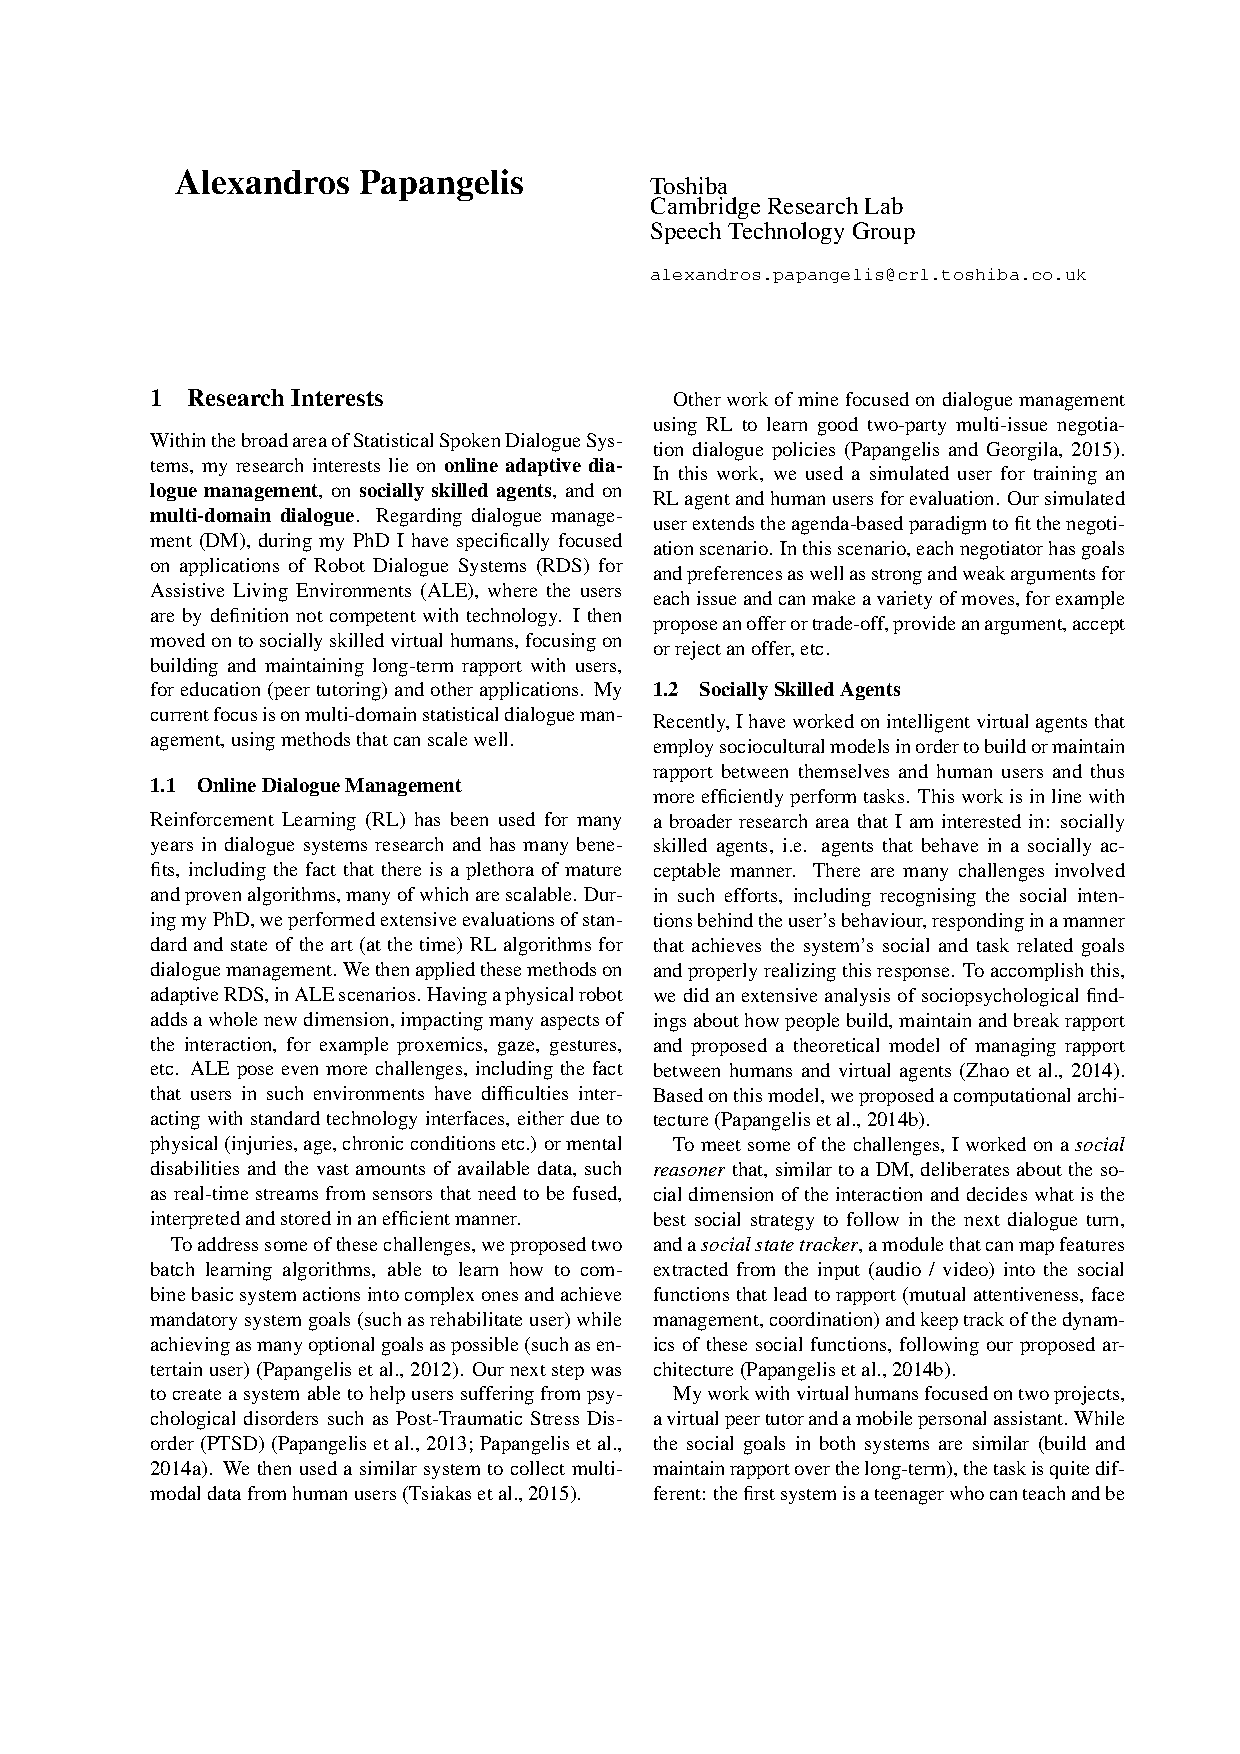
\includepdf[pages=-,pagecommand={}]{YRRSDS_2016_paper_18_alexandros_papangelis.pdf}
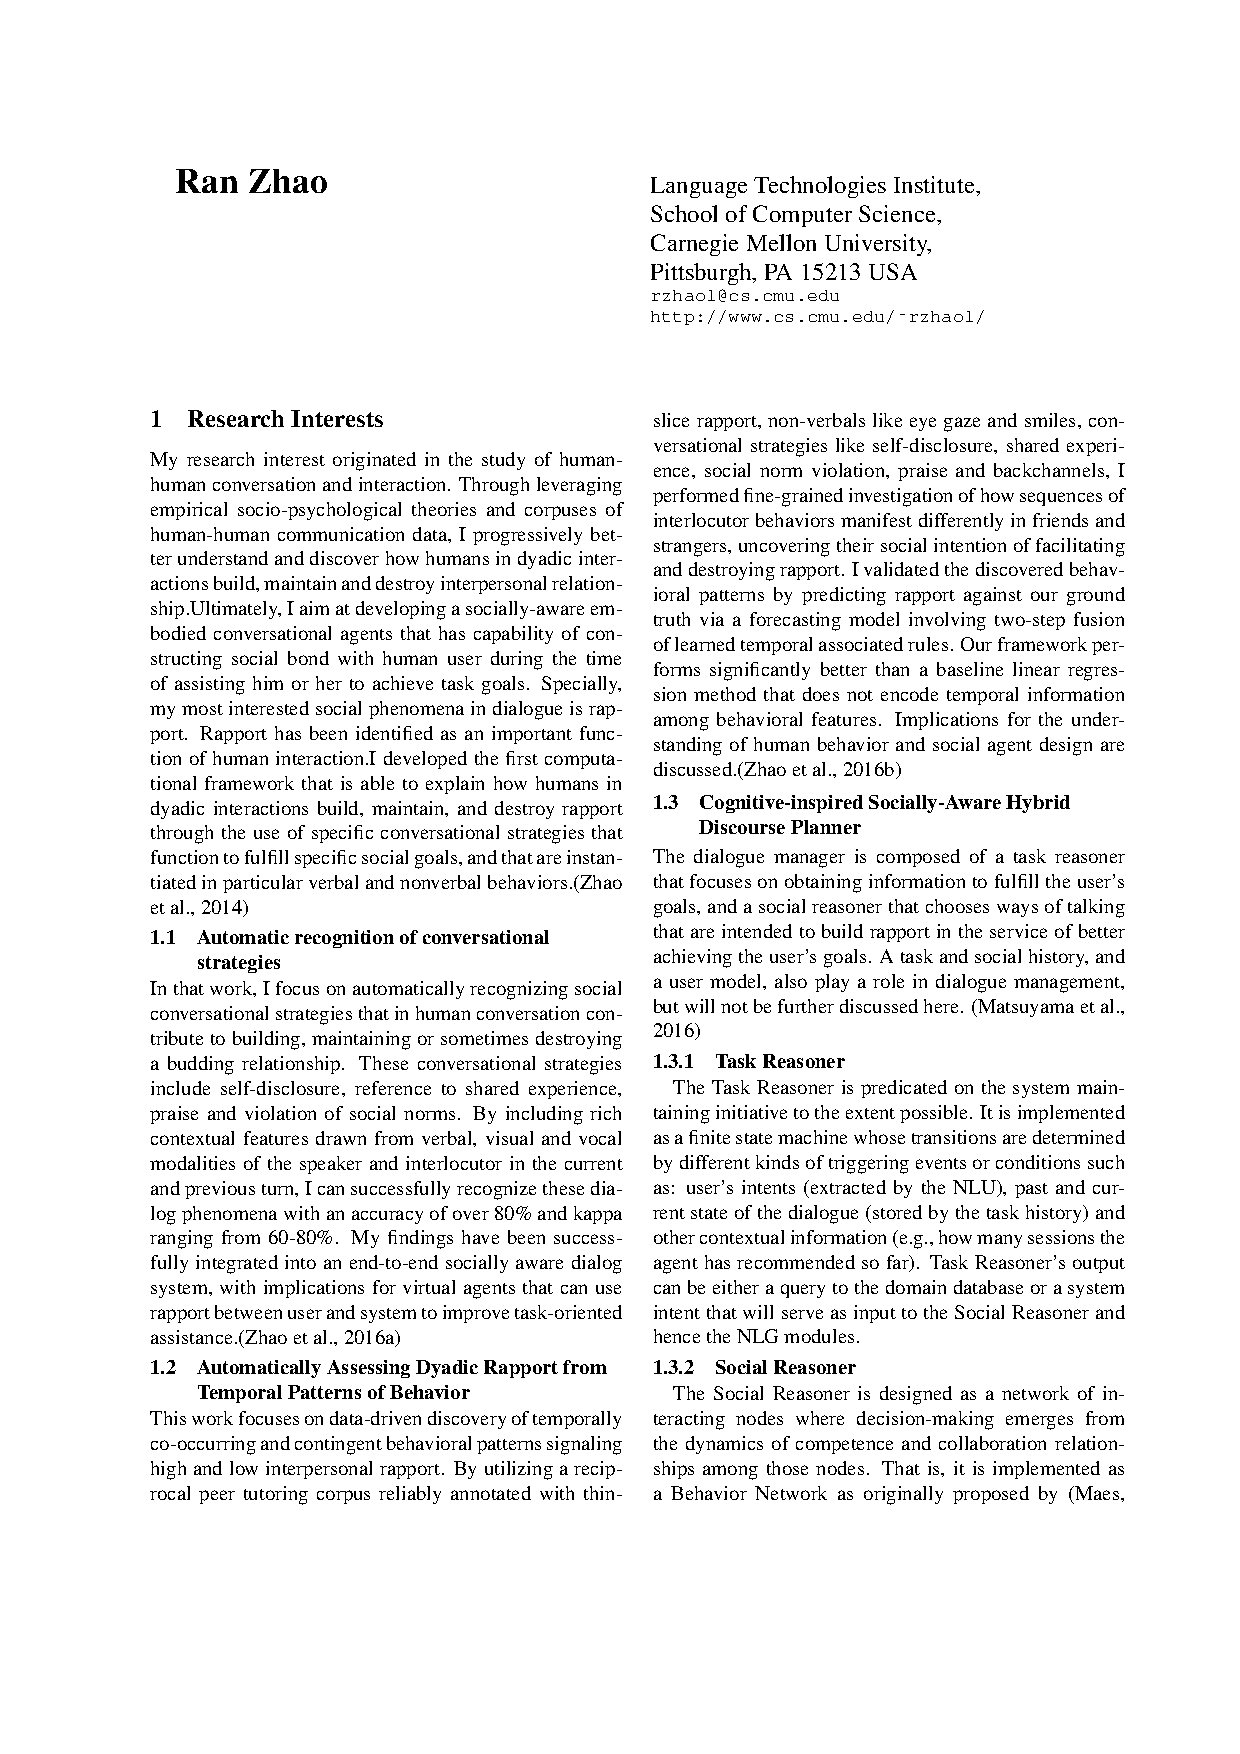
\includepdf[pages=-,pagecommand={}]{YRRSDS_2016_paper_19_ran_zhao.pdf}
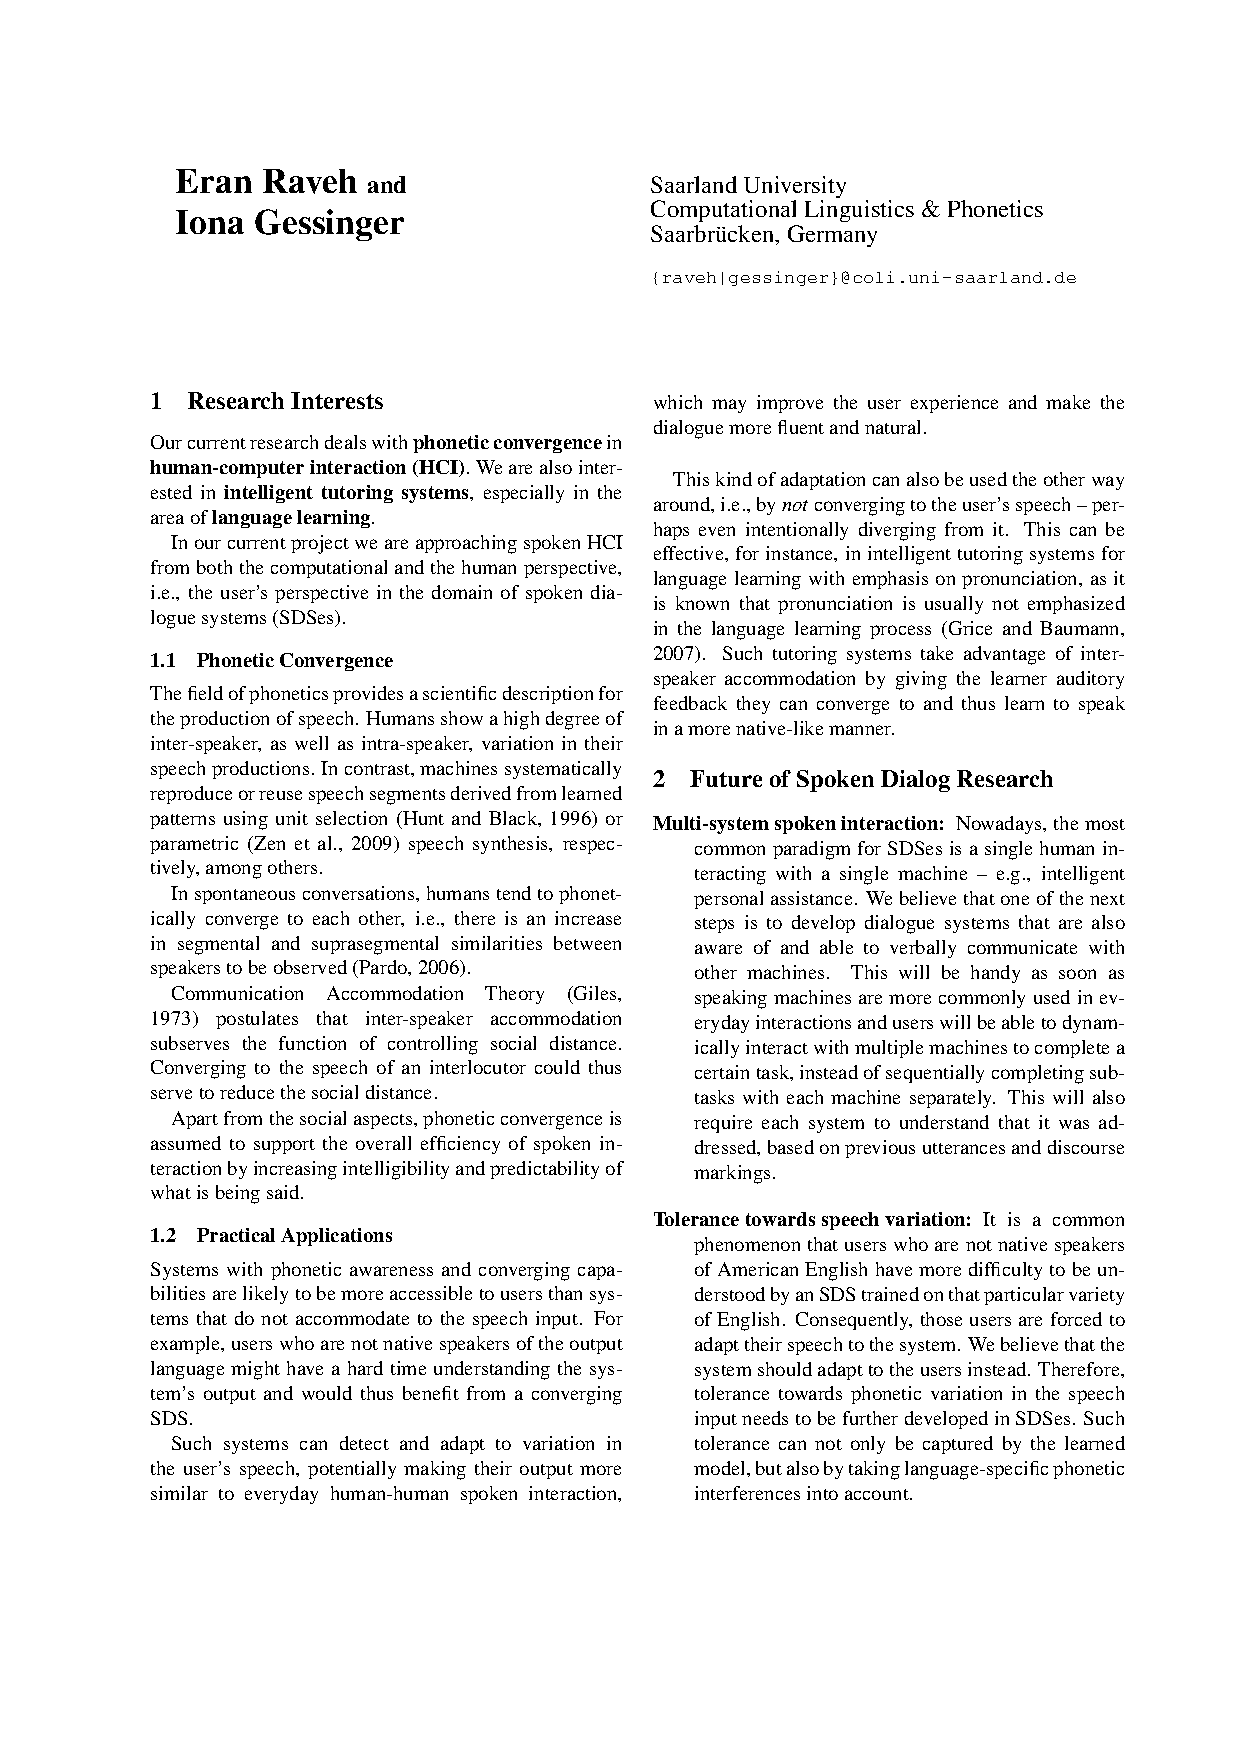
\includepdf[pages=-,pagecommand={}]{YRRSDS_2016_paper_20_eran_raveh_iona_gessinger.pdf}
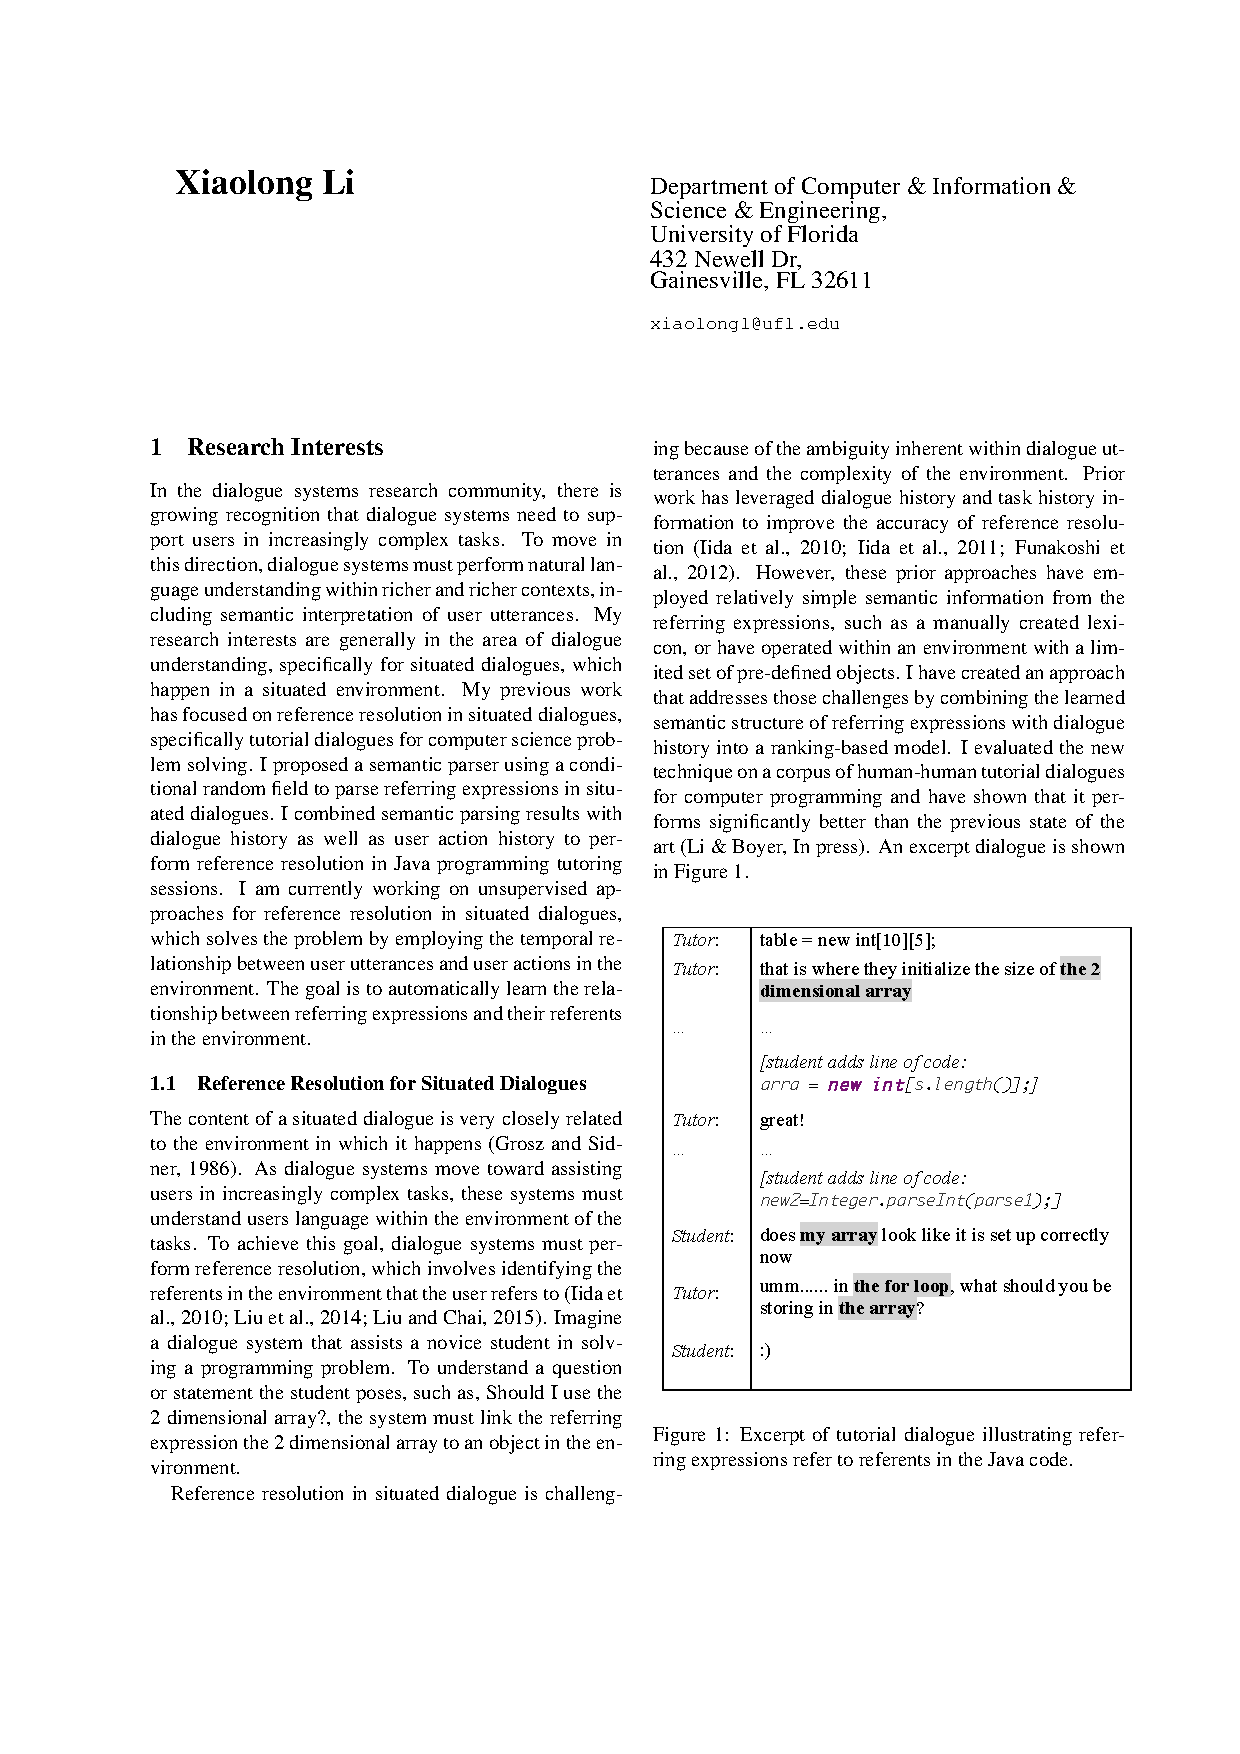
\includepdf[pages=-,pagecommand={}]{YRRSDS_2016_paper_21_xialolong_li.pdf}
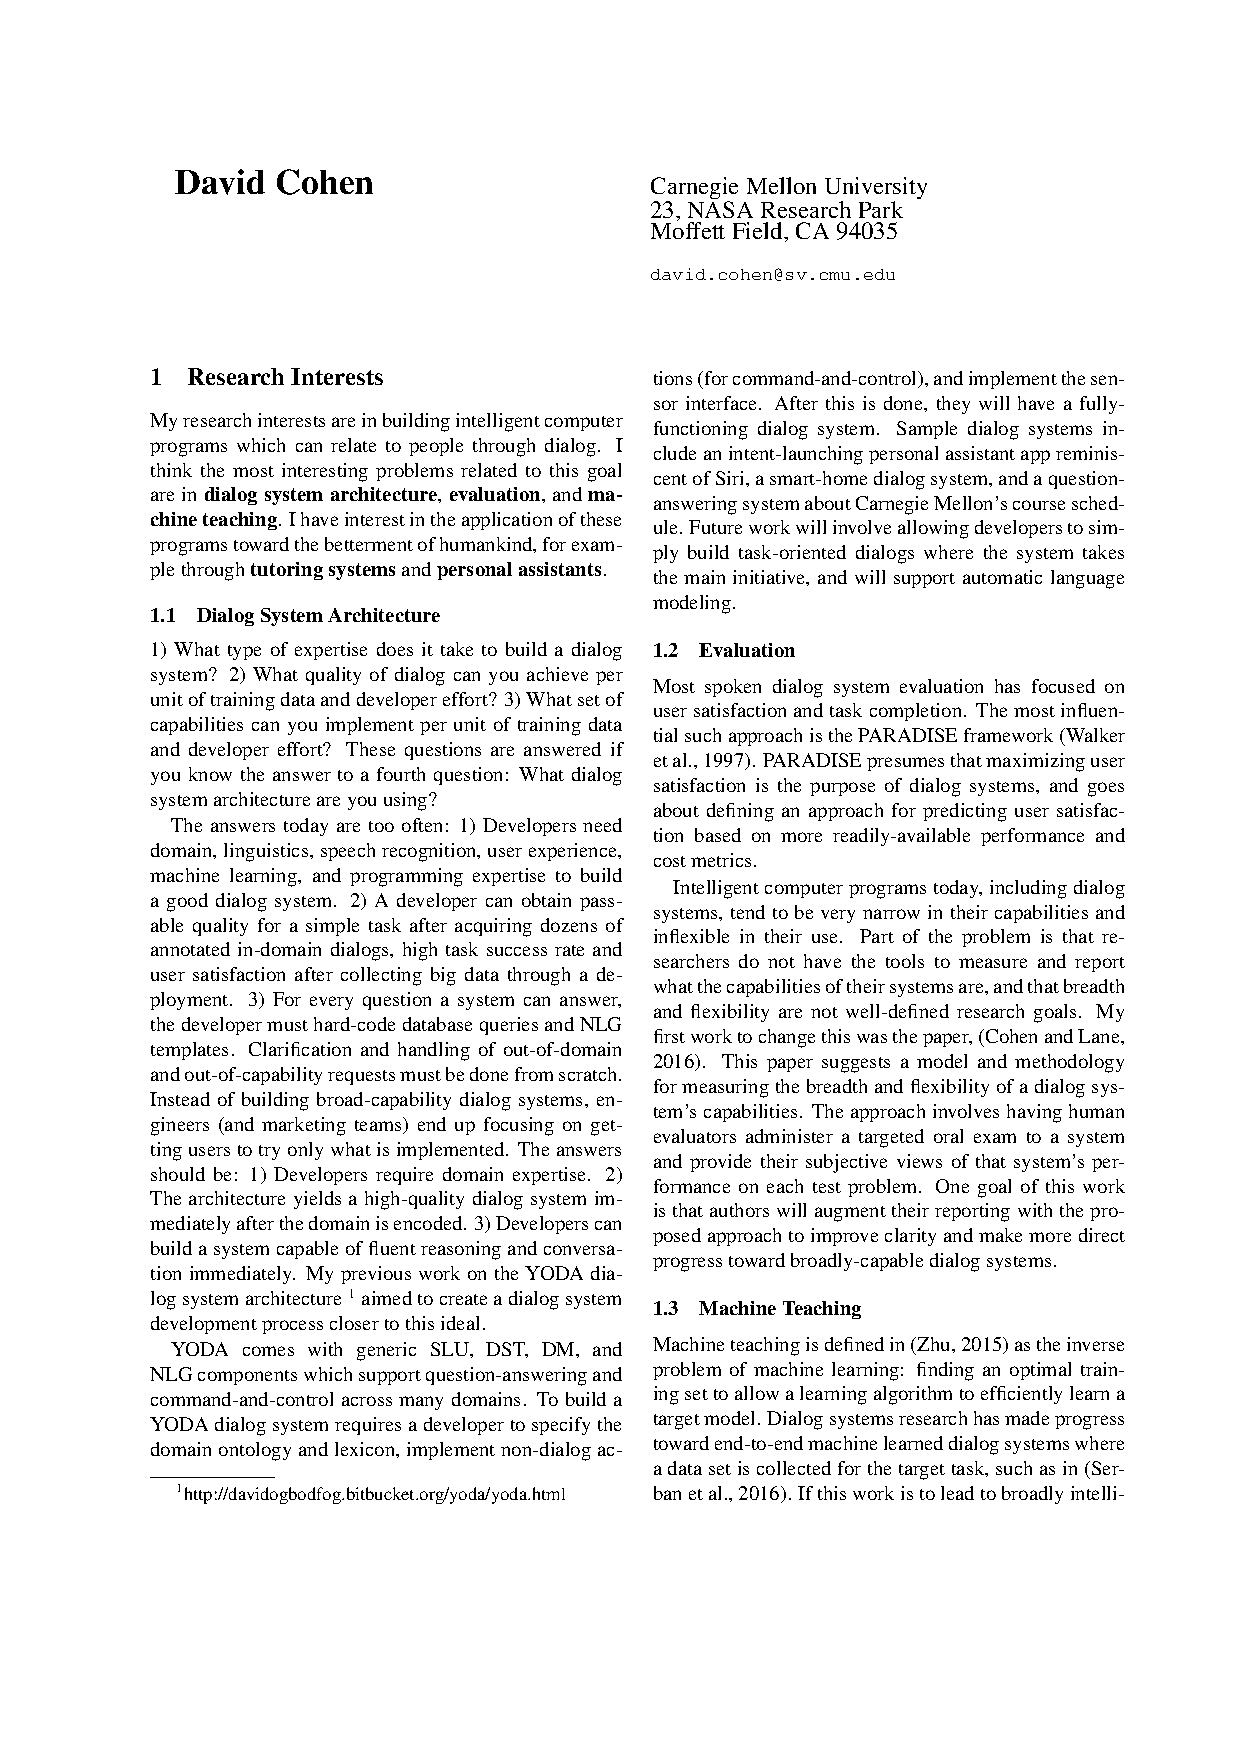
\includepdf[pages=-,pagecommand={}]{YRRSDS_2016_paper_22_david_cohen.pdf}
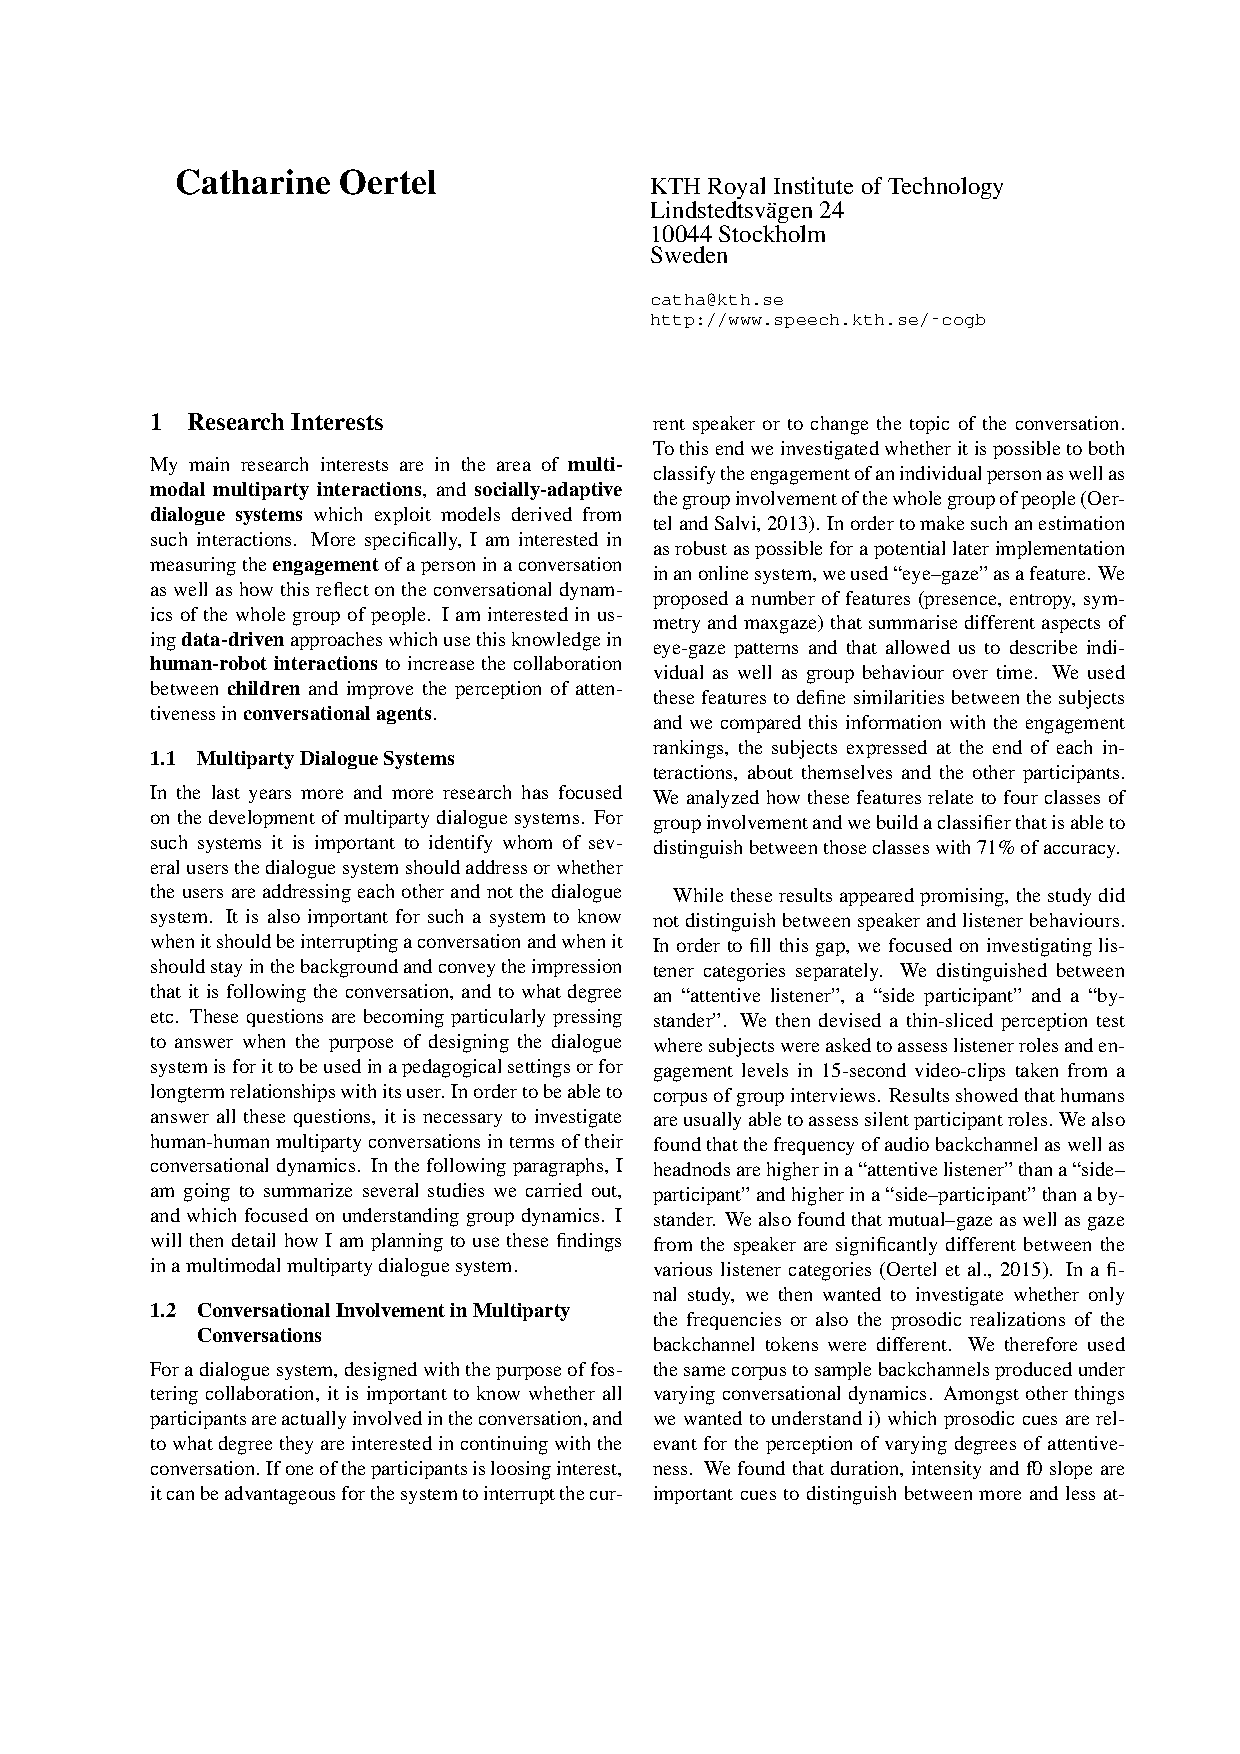
\includepdf[pages=-,pagecommand={}]{YRRSDS_2016_paper_23_catharine_oertel.pdf}
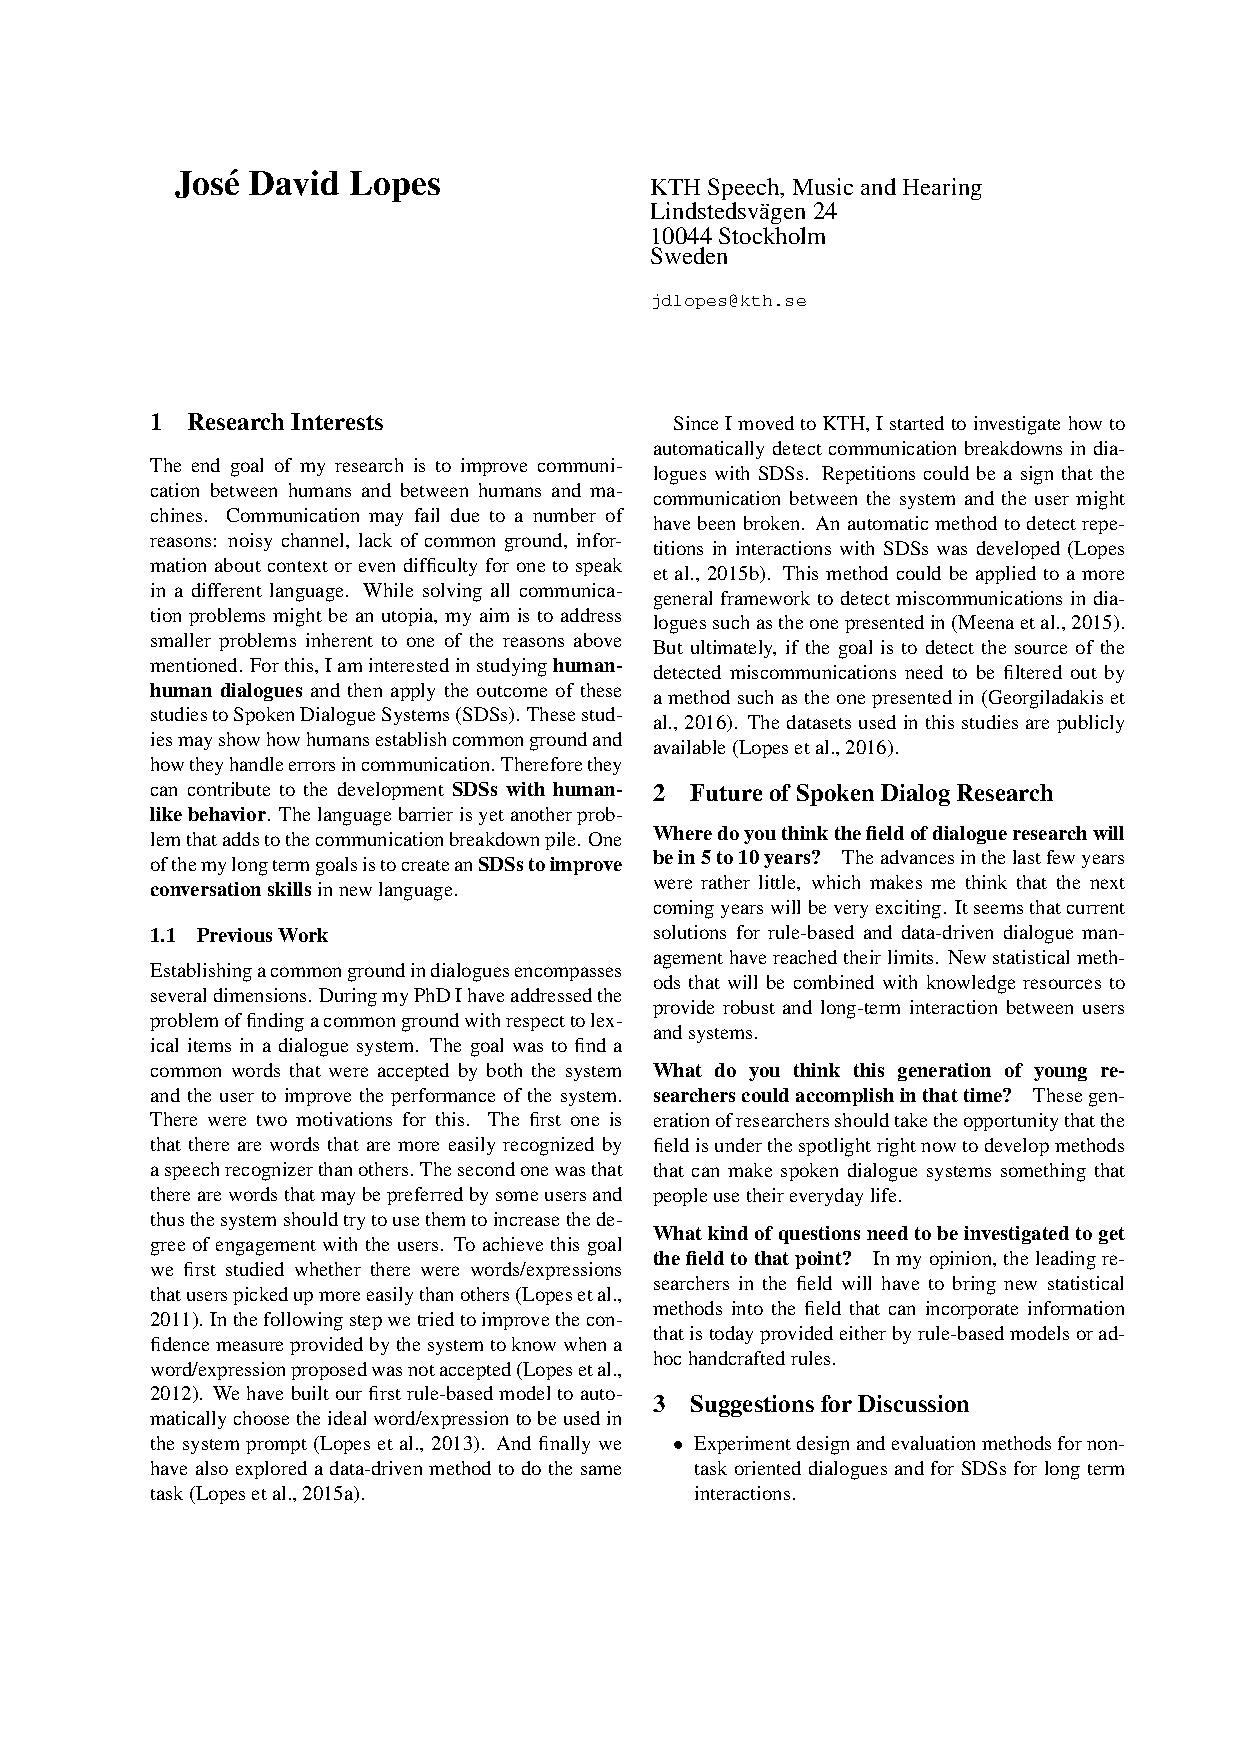
\includepdf[pages=-,pagecommand={}]{YRRSDS_2016_paper_24_jose_david_lopez.pdf}
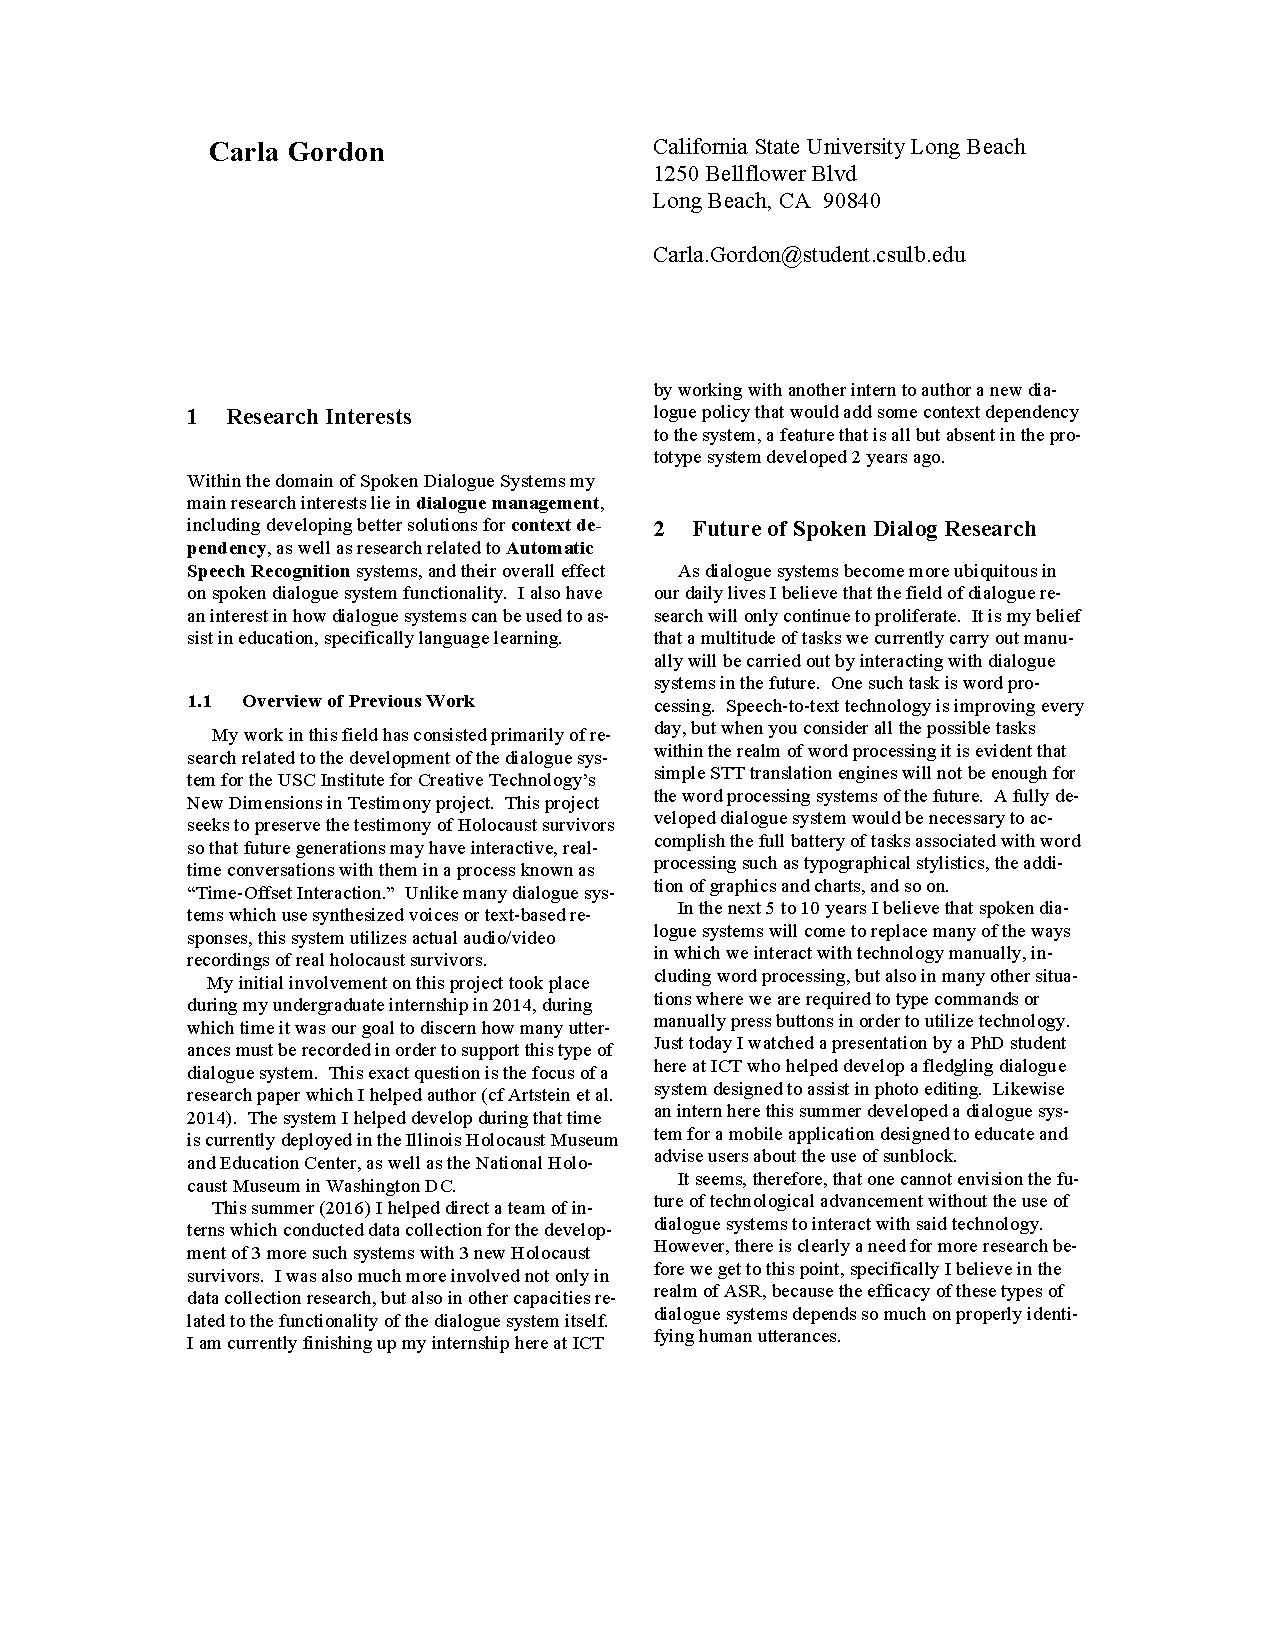
\includepdf[pages=-,pagecommand={}]{YRRSDS_2016_paper_25_carla_gordon.pdf}
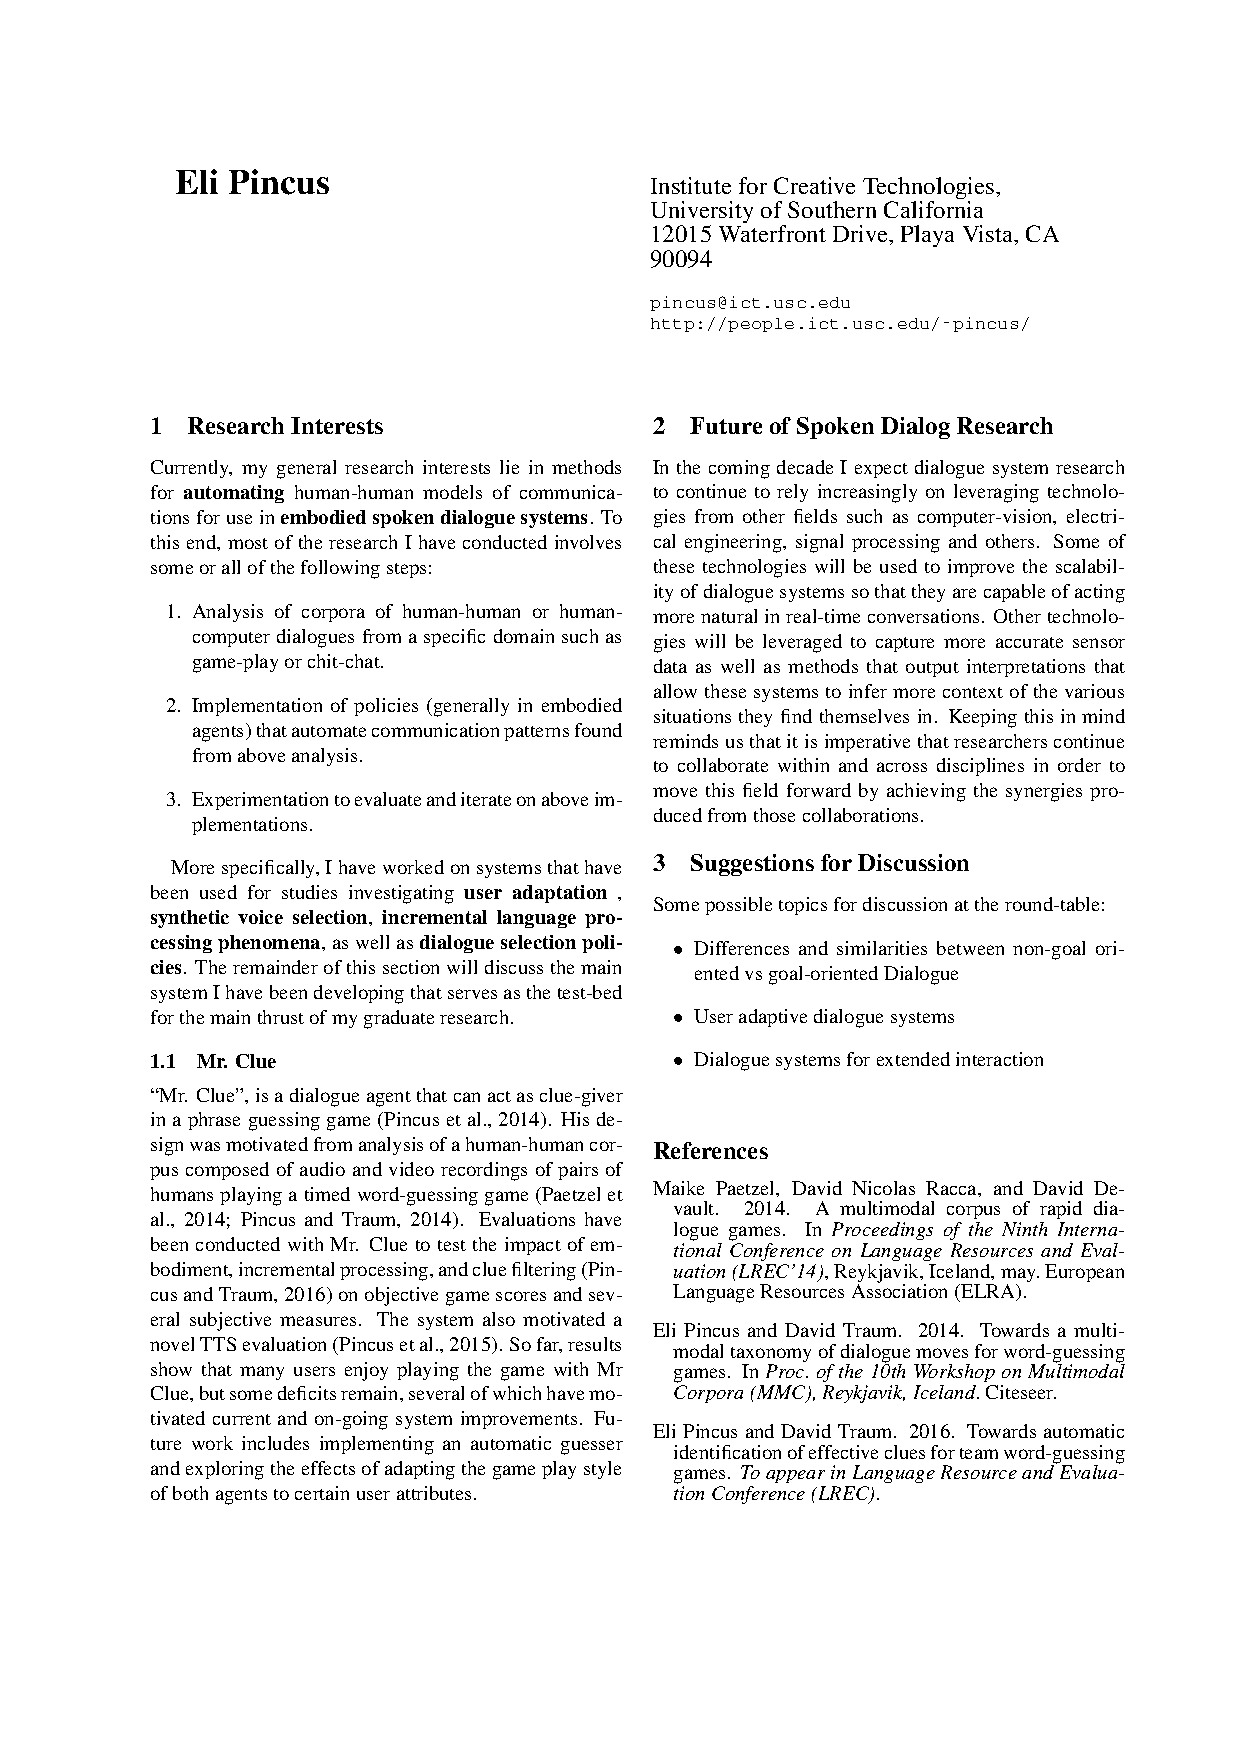
\includepdf[pages=-,pagecommand={}]{YRRSDS_2016_paper_26_eli_pincus.pdf}

% \section{Closing remarks}
% We thank all the participants for making

\end{document}
